\documentclass[12pt]{article}
\usepackage[utf8]{inputenc}
\usepackage[a4paper, margin=1in]{geometry}
\usepackage{graphicx}
\usepackage{lmodern}
\usepackage{setspace}
\usepackage{titling}
\usepackage{natbib}
\usepackage{url} % Add this line to handle URLs in bibliography
\usepackage{tabularx} % Ensure this package is loaded for extended table functionality
\usepackage{ltablex}
\usepackage{longtable}
\usepackage{array}
\usepackage{amsmath} % Add this line to handle mathematical symbols and environments
\usepackage{float}
\keepXColumns

\begin{document}
\begin{titlepage}
    \centering
    \vspace*{1cm}
    
    \Huge
    \textbf{Supplementary File for EPQ}
    
    \vspace{0.5cm}
    
    \vspace{1.5cm}
    {\Large Camron Short\par}
    {\large Candidate Number: 6439\par}
    {\large Centre Number: 19216\par}
    \vfill
\end{titlepage}

\section{Project Origins and Intellectual Context}

\subsection{Initial Curiosity}

My initial engagement with $P$ vs $NP$ was driven by genuine curiosity, not a technical understanding.
At the beginning of the project, I only knew the formal definition of the Problem and a historical tale that John von Neumann --- a mathematician who I idolise --- was told about the problem on his death bed.
The apparent simplicity of the problem's statement stood in sharp contrast to its overwhelming reputation inside the mathematical community.
I did not understand why the problem remained unsolved so I set out to learn why.
Rather than attempting to solve the problem, I attempted to develop as a mathematician by understanding why the problem has resisted solution, and more importantly, how this resistance manifests.

\section{Initial Ideas Planning}
My initial idea for the EPQ originated from a long-standing curiosity about the $P$ vs $NP$ problem.
At this stage, my understanding of the problem was extremely limited.
I knew only its formal definition: that it asks whether every problem whose solutions can be verified in polynomial time can also be solved in polynomial time.
I did not understand why this question was difficult, nor what mathematical structures were involved.
Before committing to this topic, I briefly considered alternative project ideas, including:
\begin{itemize}
    \item An exploration of Gödel's Incompleteness Theorems
    \item A study of cryptography and modern encryption systems
    \item An investigation into the mathematics of Artificial intelligence
\end{itemize}
However, each of these topics either felt too historically descriptive or too application-focused, and as someon ehoping to enter a theoretical profession i felt i would benefit more from something more abstract.
What distinguished $P$ vs $NP$ was that it appeared to be a foundational structural question about computation itself.
It did not concern a particular application, but rather the limits of efficient reasoning.
The deciding factor in choosing this topic was the contrast between the simplicity of its statement and the magnitude of its reputation.
The problem is widely described as one of the most important open questions in mathematics, and is designated as a Millennium Prize Problem by the Clay Mathematics Institute.
This combination of accessibility and depth made it both intellectually compelling and appropriately ambitious for an EPQ.
At the planning stage, my guiding question was still broad: “Why has $P$ vs $NP$ not been solved?” I did not yet anticipate that the answer would involve structural barriers such as relativisation, natural proofs, and algebrization.
The refinement of the question occurred later in the research process.

\section{Initial Ideas Planning and Mind Map}

Before beginning structured research, I explored the topic of \textit{P vs NP} through broad conceptual questioning. At this stage, my understanding was limited to the basic statement of the problem: whether every problem whose solution can be verified efficiently can also be solved efficiently. I did not yet understand the technical depth of complexity theory, nor the existence of structural barriers.

The purpose of the initial mind map was to explore possible directions the project could take, consider alternative themes, and identify which areas appeared most compelling or feasible. Rather than beginning with a fixed dissertation structure, this visual exploration allowed ideas to develop organically.

\begin{figure}[H]
    \centering
    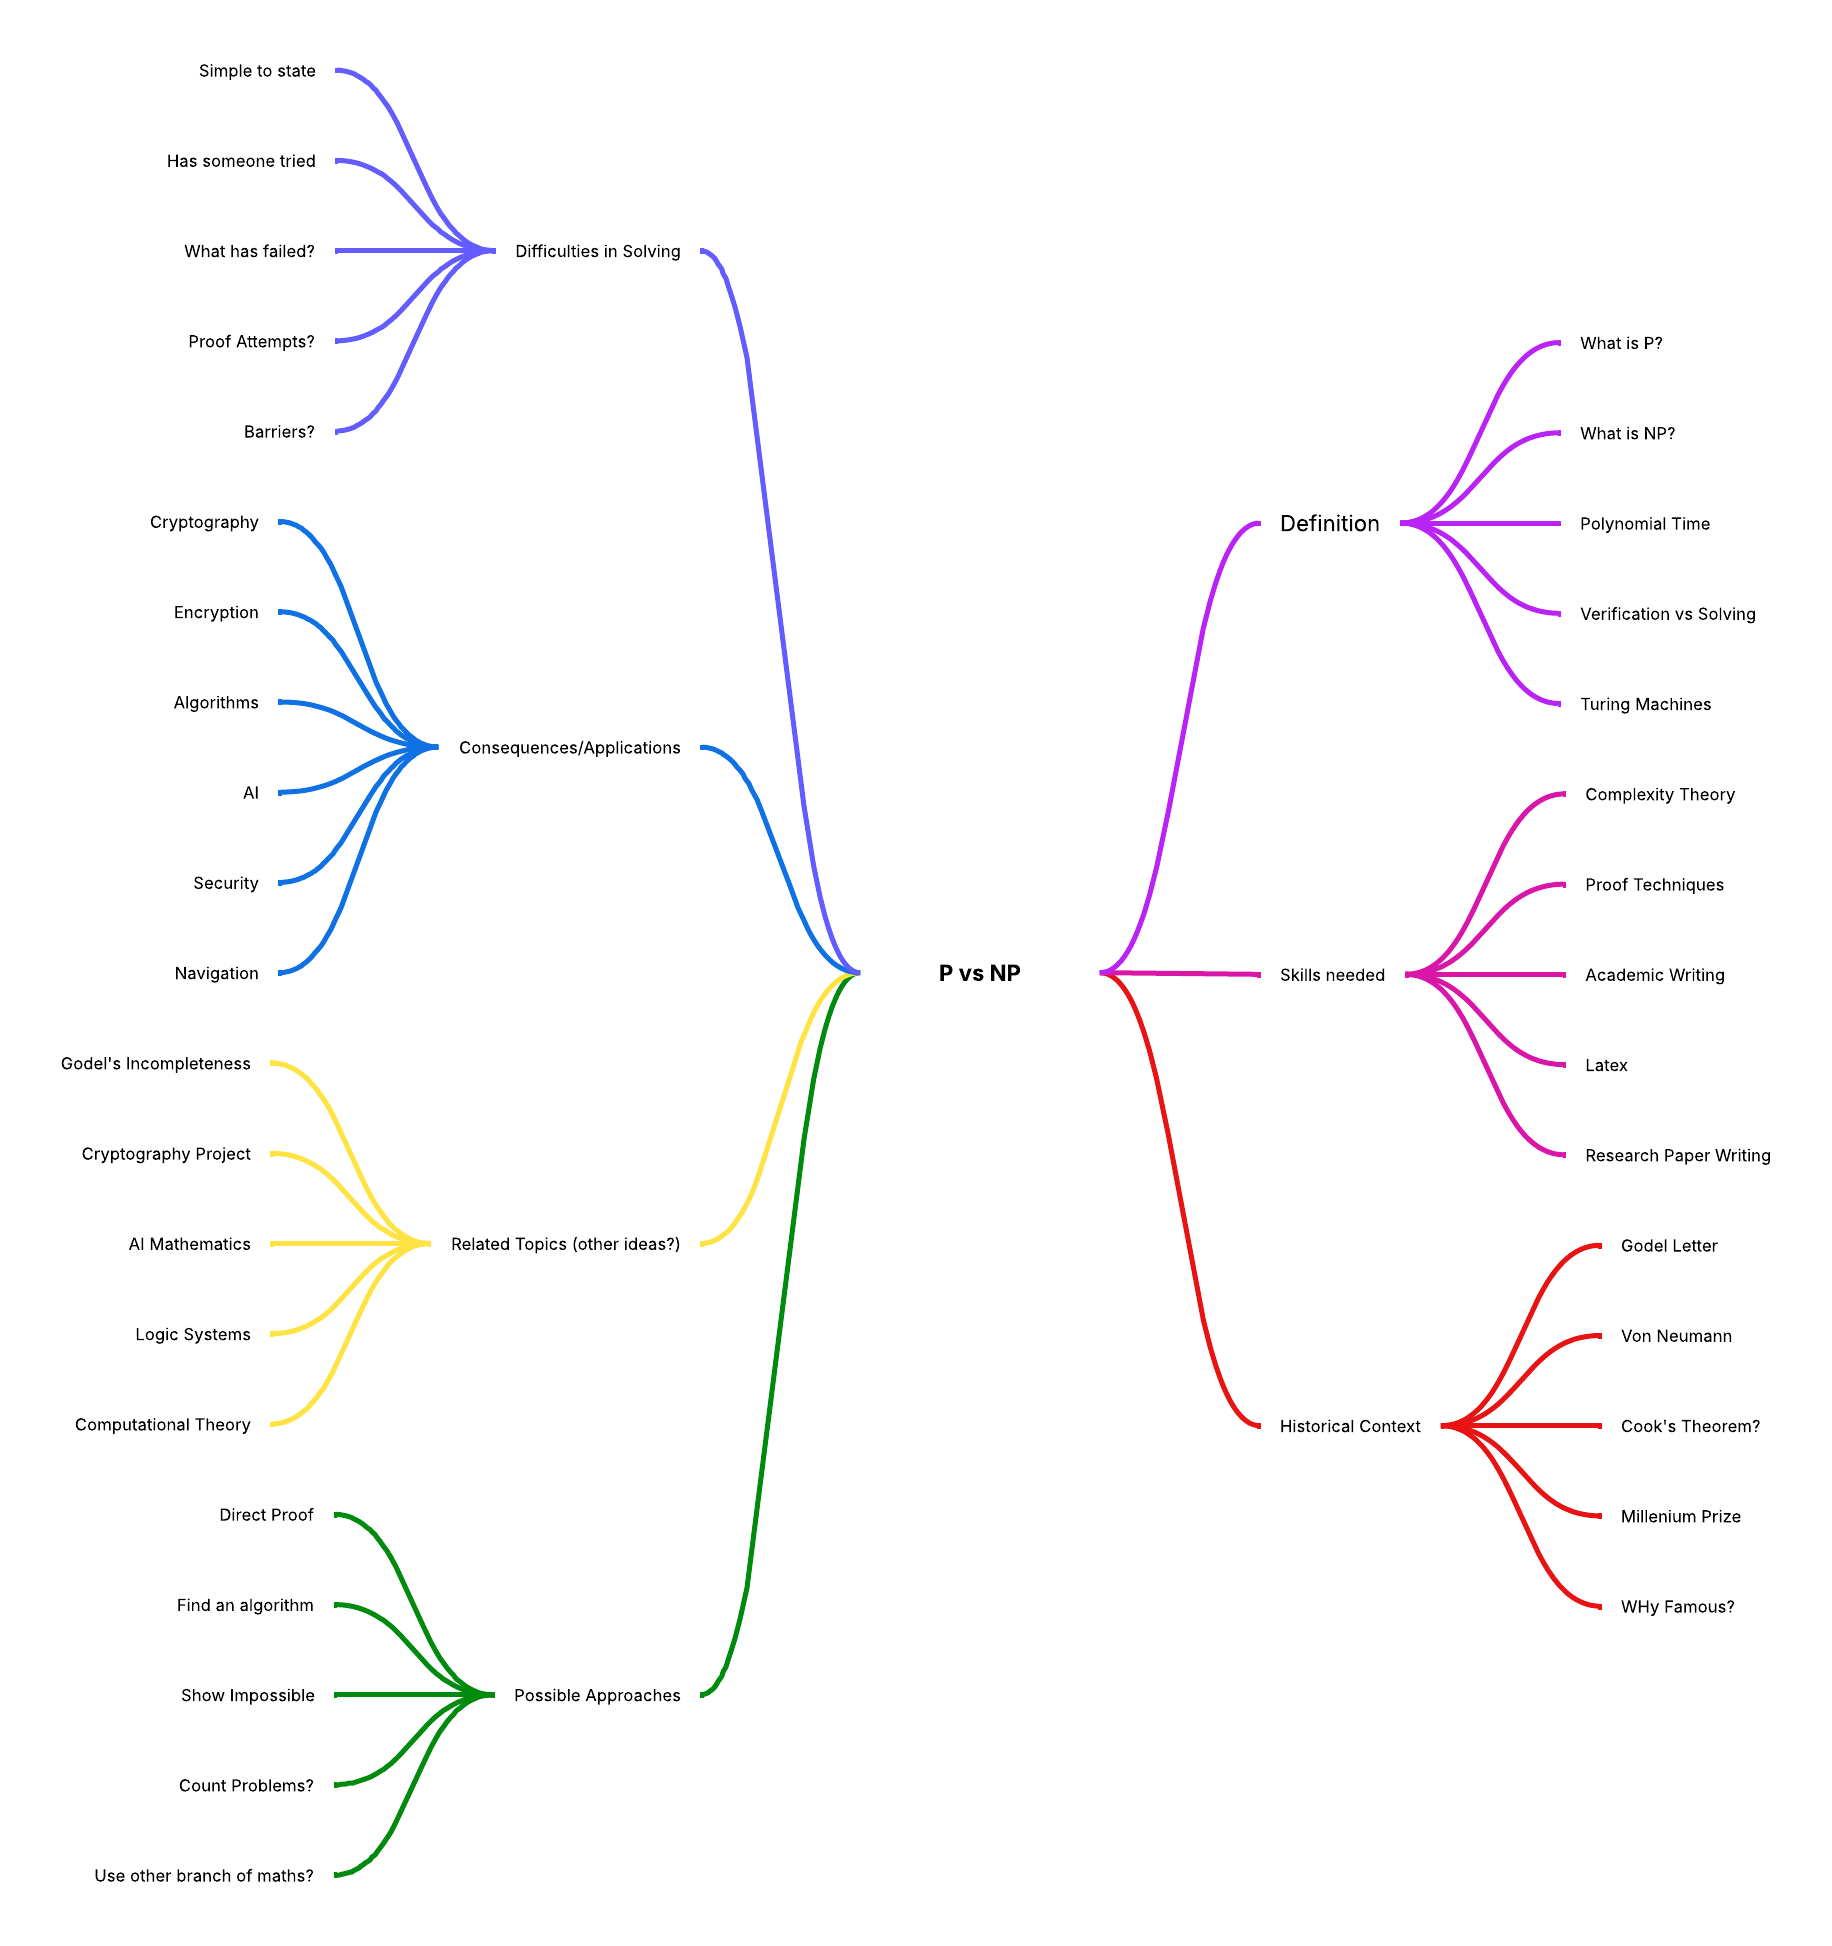
\includegraphics[width=0.85\textwidth]{MindMap.png}
    \caption{Initial exploratory mind map created before structured research began.}
\end{figure}

The central node focused on the question “Ideas for P vs NP on my EPQ”.
Surrounding branches included: foundational definitions (P, NP, polynomial time), historical context (Gödel's letter, Cook's theorem, the Millennium Prize), possible applications (cryptography, algorithms, artificial intelligence), speculative proof approaches, and related alternative topics such as Gödel's Incompleteness Theorems or encryption systems.
At this early stage, ideas were intentionally broad and in some cases naive.
For example, I briefly considered whether structural growth arguments or analogies to calculus might provide insight.
These speculative branches were later refined or discarded as research revealed the existence of formal barrier results such as relativisation, natural proofs, and algebrization.
The mind map therefore documents genuine exploratory thinking rather than retrospective structuring.
It illustrates the evolution from curiosity-driven questioning to a focused investigation of theoretical proof limitations.
This transition from broad exploration to precise framing formed the foundation of the project's development.

\subsection{Refinement of the Research Question}

The working title evolved from a broad investigation of $P$ vs $NP$ into a more precise study of the theoretical barriers preventing resolution.

After studying primary literature, it became clear that three major barriers structure modern understanding:

\begin{itemize}
\item Relativisation
\item Natural Proofs
\item Algebrisation
\end{itemize}

The dissertation therefore refined its guiding question to:

\textit{Why have existing proof techniques failed to resolve $P$ vs $NP$, and what do known barriers reveal about the structure of the problem?}

This refinement marked a significant shift from exploratory speculation toward structured engagement with established research.

\section{Initial Research Plan}

Following the exploratory mind map, the next stage was to construct a broad research plan.
At this point, the final structure of the dissertation was not determined.
The aim was instead to build foundational understanding before narrowing the research question.

\subsection*{Phase 1: Establishing Foundations}

The first objective was to understand the formal definitions of P and NP, including:
\begin{itemize}
    \item Polynomial time and asymptotic notation
    \item Decision problems and formal language theory
    \item Deterministic and non-deterministic Turing machines
    \item NP-completeness and reductions
\end{itemize}

This phase focused on textbooks and introductory material to ensure conceptual clarity before approaching research papers.

\subsection*{Phase 2: Historical and Conceptual Context}

The second stage aimed to understand how the problem developed historically and why it became central to theoretical computer science. This included:
\begin{itemize}
    \item Gödel's 1956 letter
    \item Cook's formalisation of NP-completeness
    \item Karp's expansion to combinatorial problems
    \item The designation of P vs NP as a Millennium Prize Problem
\end{itemize}

At this stage, the working research question remained broad: 
\textit{Why has P vs NP resisted solution for so long?}

\subsection*{Phase 3: Investigating Failed Approaches}

Only after building foundational understanding did the plan include exploring previous attempts or methodological obstacles.
The intention was to identify patterns in failed approaches rather than attempt an original proof.

This stage was initially undefined and exploratory.
It was not yet clear whether resistance to solution was due to technical difficulty, philosophical limits, or structural features of complexity theory.

\subsection*{Planned Outcome (Early Stage)}

The intended outcome was a dissertation.
However, the precise structure was deliberately left flexible.
The research plan prioritised understanding and refinement of the question over early commitment to a rigid chapter framework.
This allowed the project direction to evolve naturally as deeper literature was encountered.

\section{Project Timeline and Development}

A timeline was created at the beginning of the project to structure research, drafting, and presentation stages.
The initial plan divided the project into broad phases: foundational learning, literature review, drafting, revision, and preparation for the exhibition.

Unlike a fixed blueprint, the timeline was designed to be adaptive.
As research progressed, it became clear that certain areas required substantially more time than originally anticipated, particularly the Natural Proofs chapter and the prerequisite study of circuit complexity.
The timeline was therefore adjusted to reallocate time toward deeper conceptual understanding rather than early drafting.

\subsection*{Initial Timeline Structure}

The early timeline was organised into the following stages:

\begin{itemize}
    \item Weeks 1--3: Foundational research (definitions, NP-completeness, reductions)
    \item Weeks 4--6: Historical context and overview of proof attempts
    \item Weeks 7--9: Investigation of methodological obstacles
    \item Weeks 10--12: Drafting of dissertation
    \item Weeks 13--14: Editing, formatting, and preparation for presentation
\end{itemize}

At this stage, the research question remained broad, and the specific barrier framework had not yet been fully identified.

\subsection*{Adaptation and Refinement}

As primary research papers were encountered, particularly those concerning Natural Proofs and algebrization, the timeline required revision.
The technical density of these topics necessitated a temporary pause in drafting to study Boolean circuits and pseudorandom functions in greater depth.
This adjustment extended the research phase but significantly improved conceptual accuracy.

Additionally, time was allocated to skill development, including learning \LaTeX{} for mathematical typesetting and using Manim to generate graphical illustrations.
These technical tasks were not part of the original schedule but became necessary to improve clarity and presentation quality.

The evolving timeline therefore reflects the non-linear nature of research. Rather than following a rigid sequence, the project developed iteratively, with research informing structure and structure informing further research.

\subsection*{Reflection on Time Management}

Overall, the timeline functioned as a structural guide rather than a strict constraint. While some phases required extension, early planning prevented major delays and ensured steady progress toward completion. The most significant lesson from this process was that advanced theoretical topics often require disproportionately more time for comprehension than for writing. Recognising this early prevented rushed analysis and allowed the final dissertation to prioritise conceptual precision over superficial coverage.
The original version of the timeline has been retained as evidence of initial planning, while the revised version reflects adjustments made during the research process.
Comparing the two illustrates how the scope of the project narrowed from broad conceptual curiosity to a focused analysis of theoretical proof barriers.

\section{Planning and Timeline Commentary}

\subsection{Initial Planning Assumptions}

At the outset of the project, I underestimated the conceptual complexity of primary research papers within computational complexity theory. I initially believed that reading foundational papers directly would accelerate understanding of the problem's structure.

This assumption proved incorrect. 
The technical density of works such as Baker-Gill-Solovay and Razborov-Rudich required prerequisite knowledge in areas such as oracle constructions, circuit complexity, and pseudorandom functions, which I had not yet consolidated.

The original plan therefore underestimated the amount of foundational consolidation required before engaging with barrier literature.

\subsection{Adaptive Strategy and Reallocation of Time}

After encountering substantial difficulty with the Natural Proofs paper in particular, I paused direct engagement with primary sources and shifted to structured study of prerequisite material, including:

\begin{itemize}
    \item Boolean circuit models and circuit lower bounds
    \item Polynomial-time reductions
    \item Interactive proof systems
    \item Arithmetisation techniques
\end{itemize}

This tactical pause significantly improved subsequent comprehension and prevented superficial reading.

The Gantt chart reflects this shift, showing extended time allocation for the Natural Proofs and Algebrisation chapters compared to initial estimates.

\subsection{Weekly Checkpoints (Aligned to Gantt Chart)}

The following summaries reflect the weekly monitoring of the project in direct alignment with the Gantt chart.
Although supervisory meetings followed standard EPQ structure, I used them as structured checkpoints to evaluate intellectual progress, depth of understanding, and necessary timeline adjustments.

\subsubsection*{Week 1 --- Proposal and Scope Definition (Late October)}

Focus: Refinement of research question and feasibility.

Discussion centred on narrowing the project from a broad investigation of $P$ vs $NP$ to a focused study of known proof barriers.
At this stage, understanding was introductory, and the primary objective was ensuring that the scope was realistic within the word limit.

Action taken: Finalised proposal and constructed Gantt chart.

Reflection: This was a structural phase rather than a technical one.
The key development was recognising that attempting to "solve" the problem would weaken the academic credibility of the project.

\subsubsection*{Week 2 --- Foundational Concepts (Early November)}

Focus: Definitions and technical precision.

Work involved clarifying $O(n)$ notation, defining $P$ and $NP$ formally, and refining the research question.
Supervisor emphasis was on mathematical accuracy and clarity of communication.

Action taken: Rewrote definitions using formal notation and removed informal phrasing.

Reflection: Began understanding that mathematical writing must prioritise precision over explanation.

\subsubsection*{Week 3 --- Introduction to Relativisation (Mid November)}

Focus: Understanding oracles and Turing machines.

Although the concept of an oracle initially appeared simple, I struggled with understanding how the Baker-Gill-Solovay proof was constructed.

Action taken: Paused forward progression to consolidate understanding of oracle Turing machines.

Reflection: This marked the first instance where intellectual depth required schedule adjustment.

\subsubsection*{Week 4 --- Deepening Relativisation (Late November)}

Focus: Implications of relativisation.

Discussion examined what it means for a proof technique to relativise and whether my early structural ideas would also relativise.

Action taken: Incorporated explicit evaluation of whether my derivative framework relativises.

Reflection: This stage shifted my thinking from speculative ideas to structural validity.

\subsubsection*{Week 5 --- Natural Proofs (Early December)}

Focus: Circuit complexity and the structure of the Razborov-Rudich argument.

I realised I lacked foundational understanding of Boolean circuits, which prevented meaningful engagement with the paper.

Action taken: Reallocated time to study circuit complexity and pseudorandom functions before continuing.

Reflection: This was a major intellectual difficulty phase and required deliberate slowing of progress.

\subsubsection*{Week 6 --- Consequences of Natural Proofs (Mid December)}

Focus: Cryptographic implications and barrier interpretation.

Discussion centred on understanding what Natural Proofs actually prohibit and avoiding exaggerated claims about its strength.

Action taken: Refined wording to ensure accurate representation of the barrier.

Reflection: Mathematical maturity noticeably improved during this phase.

\subsubsection*{Week 7 --- Algebrization Foundations (Late December)}

Focus: Arithmetisation and interactive proofs.

Study included Shamir's IP = PSPACE result and algebraic extensions of Boolean functions.

Action taken: Consulted prerequisite material selectively to avoid unnecessary technical overload.

Reflection: Conceptual comprehension was stronger than in earlier chapters due to accumulated experience.

\subsubsection*{Week 8 --- Development of Personal Investigation (Early January)}

Focus: Evaluating inclusion of derivative-based framework.

Discussion centred on whether including an independent attempt would strengthen or weaken the dissertation.

Action taken: Included the attempt with explicit limitations and critical evaluation.

Reflection: Ensured the investigation supported rather than detracted from the core thesis.

\subsubsection*{Week 9 --- Technical Presentation (Mid January)}

Focus: Learning \LaTeX{} and Manim for professional presentation.

Action taken: Implemented formal formatting and generated graphical illustration for personal attempt.

Reflection: Technical development enhanced clarity and academic presentation quality.

\subsubsection*{Week 10 --- Finalisation and Evaluation (Late January --- February)}

Focus: Word count reduction and structural refinement.

Action taken: Strengthened evaluative commentary and ensured all sections aligned directly with the refined research question.

Reflection: The final phase emphasised communication efficiency over new knowledge acquisition.

\subsection*{Overall Monitoring Reflection}

The weekly checkpoints demonstrate a progression from structural planning to deep technical engagement and finally to evaluative refinement. Deviations from the initial schedule were deliberate responses to intellectual difficulty rather than poor planning, and each adjustment strengthened the overall academic integrity of the project.

\subsection*{Gantt Chart and Timekeeping}
The project was structured using a Gantt chart to manage phases of research, technical development, drafting, and revision.
\begin{figure}[H]
    \centering
    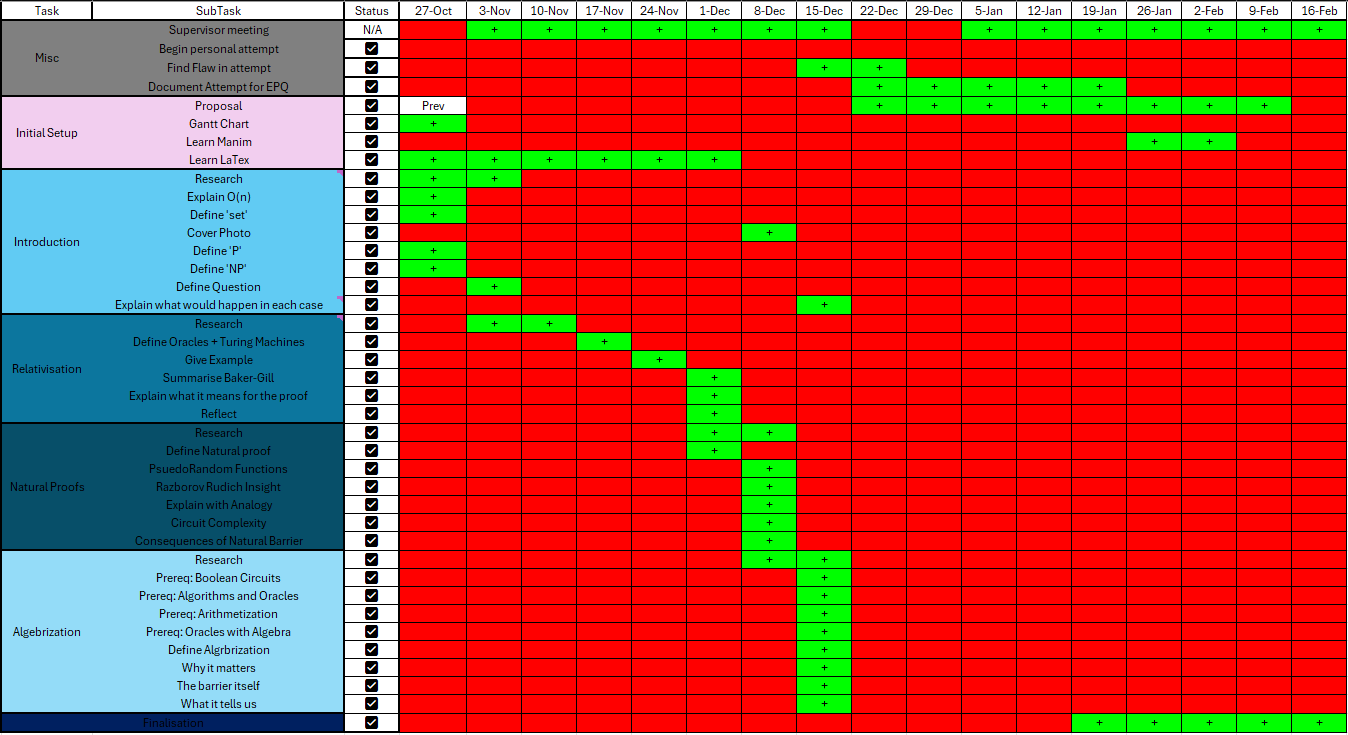
\includegraphics[width=1.1\textwidth]{Gantt.png}
    \caption{Gantt chart outlining planned and completed phases of research and drafting.}
    \label{fig:gantt}
\end{figure}

The Gantt chart illustrates the planned and realised progression of the project across separate phases: foundational consolidation, barrier-focused research, independent exploration, and final drafting.

\subsubsection*{Initial Setup and Primary Phase}

The early weeks (late October to mid-November) were allocated to introductory consolidation, including defining $P$, $NP$, set-theoretic foundations, and learning \LaTeX. 

This phase proceeded largely as planned. The structured development of definitions and background material created a necessary base before engaging with primary research papers. The chart displays consistent weekly progress in this period, reflecting steady core work.

However, the initial attempt to interact directly with primary literature occurred earlier than ideal. Although ambitious, this decision revealed gaps in prerequisite knowledge and ultimately necessitated later reallocation of time.

\subsubsection*{Relativisation and Natural Proofs Phase}

The most significant deviation since initial planning occurred during the Natural Proofs and Relativisation chapters (late November through mid-December).

While Relativisation progressed in a relatively contained timeframe, the Natural Proofs section expanded beyond its original allocation. This extension was due to the unexpected conceptual demands of circuit complexity and pseudorandom functions. 

The chart reflects this by showing a sustained period of concentrated work across multiple weeks. Rather than moving forward with partial understanding, time was deliberately reassigned to learning circuit models and non-uniform complexity in greater depth.

This phase marks a shift from linear progression to adaptive management.

\subsubsection*{Algebrisation and Prerequisite Consolidation}

The Algebrisation chapter required additional prerequisite study, particularly interactive proofs and arithmetisation. The Gantt chart indicates renewed consolidation in mid-December before full engagement with the barrier result.

Although this delayed the drafting schedule, it strengthened comprehension and prevented superficial treatment of technically demanding material.

\subsubsection*{Independent Investigation and Finalisation}

The independent, derivative-based investigation emerged following substantial engagement with the barrier literature. Its placement later in the timeline reflects intellectual maturation rather than early speculation.

The finalisation phase (January-February) shows concentrated drafting and structural refinement. This period involved significant rewriting, language compression to meet word limits, and thematic reorganisation of research notes.

\subsubsection*{Evaluation of Time Management}

The Gantt chart shows that, while the initial time estimates for primary literature were optimistic, the project remained manageable through effort reallocation.

The most important managerial development was recognising when comprehension required consolidation rather than continuation. Treating the plan as adaptive rather than rigid prevented cumulative misunderstanding.

In retrospect, beginning with survey-level framing before engaging primary barrier papers would have improved efficiency. However, confronting technical material early accelerated familiarity with the language of mathematical research.

Overall, the project evolved from enthusiasm-driven immersion to structured academic management. The Gantt chart reflects this transition from exploratory progression to disciplined consolidation and refinement.

\subsection{Monitoring Progress and Self-Regulation}

Progress was monitored through periodic review of the Gantt chart and written consolidation of research notes after each major reading phase. 

When comprehension difficulties arose --- particularly during the Natural Proofs chapter --- I avoided continuing without understanding and instead paused to consolidate prerequisite knowledge. This decision prevented shallow engagement and ensured that later chapters were built upon secure foundations.

Rather than following the original timeline, I treated the plan as flexible. When foundational gaps were identified, the priority shifted to conceptual consolidation before returning to the primary literature. 

This repeated monitoring process allowed the project to evolve in depth without sacrificing coherence.

\subsection*{Note on Structure}

This document was developed progressively throughout the EPQ process. 

While many research notes were written chronologically, the final organisation has been structured thematically to increase clarity and navigability. 

This restructuring process reflects the intellectual evolution of the project --- from exploratory reading toward focused engagement with complexity-theoretic barriers --- and aims to present the research process coherently while preserving evidence of development.

\subsection{Research Phases}

The first phase focused on basic understanding of complexity classes, reductions, and NP-completeness. This required consolidating knowledge from textbooks before engaging with research papers.

The second phase consisted of studying the three barrier results in chronological order, beginning with relativisation (1975), then natural proofs (1994), and finally algebrisation (2008). This order paralleled the historical development of the field and clarified how each barrier refined limitations identified by its predecessors.

\subsection{Adjustments to the Timeline}

Several adjustments were necessary during the project:

\begin{itemize}
\item The Natural Proofs chapter required significantly more time than anticipated due to the need to understand circuit complexity and pseudorandom functions.
\item Algebrisation required additional background reading on interactive proofs and arithmetisation.
\item Technical presentation tools (LaTeX and Manim) required learning time not initially budgeted.
\end{itemize}

These delays resulted in a reallocation of time from speculative exploration to structured consolidation of barrier theory.

\subsection{Supervisor Interaction and Independence}
Although supervisory meetings were largely procedural in nature and focused on EPQ administrative requirements, they provided important structural checkpoints. These meetings ensured that the project remained aligned with assessment objectives and prevented excessive deviation into excessively technical territory. While mathematical direction was self-led, supervisory input helped maintain concentration regarding clarity, organisation, and formal requirements.

\subsection{Independent Direction of Study}

Supervisor meetings focused primarily on procedural EPQ requirements rather than subject-specific guidance. Consequently, decisions regarding topic refinement, source selection, and structural organisation were made independently.

This independence required continuous self-evaluation of feasibility, scope, and academic appropriateness. While this increased the regulatory burden, it also strengthened ownership of the project's intellectual direction.

\subsection{Early Understanding and Misconceptions}

In the early stages of research, I approached the problem as if it were a particularly difficult but isolated theorem. 
However, reading introductory material quickly revealed that $P$ vs $NP$ is not simply a single question, but the centre of a vast framework involving reductions, completeness, circuit complexity, and proof systems.

The discovery of NP-completeness, particularly through Cook's theorem and Karp's reductions, demonstrated that the problem is structurally embedded across numerous combinatorial problems. 
This shifted my perception of $P$ vs $NP$ from a technical curiosity to a basic structural question about computation itself.

At this stage, I still believed the main obstacle was technical difficulty rather than theoretical limitation.

\subsection{Shift in Intellectual Direction}

The most major structural change in the project was the decision to focus not on attempting a direct resolution of $P$ vs $NP$, but on analysing the known proof barriers preventing resolution.

Initially, the problem appeared as an extremely difficult but isolated theorem. Through reading Cook and Karp, I realised that the problem is structurally embedded across wide classes of combinatorial problems via NP-completeness.

Further study of relativisation demonstrated that the difficulty is not simply technical although methodological: entire families of proof techniques have been shown to fail.

This realisation fundamentally reshaped the project's direction and strengthened its analytical focus.

\subsection{Feasibility and Scope Control}

An early risk identified was the possible overreach of attempting to contribute directly to the resolution of $P$ vs $NP$. 

Through engagement with barrier literature, it became clear that the problem is embedded within an elaborate framework of limitations on proof techniques. This recognition led to a controlled narrowing of scope: the project shifted from speculative solution attempts toward analytical study of why existing strategies fail.

This adjustment ensured that the final dissertation remained academically rigorous and realistically achievable within the constraints of the EPQ.

\subsection{Evaluation of Project Management}

In retrospect, the initial plan underestimated the depth of prerequisite knowledge required for primary complexity theory research. Beginning with survey material such as Fortnow's overview before reading primary barrier papers would have improved early comprehension efficiency.

However, the decision to confront primary literature early --- though inefficient --- accelerated familiarity with the language of mathematical research and improved long-term reading fluency.

Overall, the project management process evolved from optimistic immersion to structured consolidation. This transition demonstrates a shift from enthusiasm-driven exploration to disciplined academic strategy.

\subsection{Structural Decisions and Reorganisation}

Although this document is presented in clearly separated thematic sections (Relativisation, Natural Proofs, Algebrisation), the research process itself was not strictly linear.
In practice, I often encountered conceptual dependencies that required temporary diversion into prerequisite material before returning to the main barrier being studied.
For clarity of navigation and academic coherence, I reorganised the document into thematic blocks rather than strict chronological order.
This decision was made to prioritise conceptual accessibility for the examiner over historical sequencing.
A note has therefore been included clarifying that the document underwent structural refinement after initial drafting.
This reorganisation reflects deliberate project management rather than retrospective editing.
It demonstrates conscious adaptation in response to increasing subject complexity, particularly when Natural Proofs and circuit complexity required substantial prerequisite learning before meaningful engagement was possible.

\subsection{Supervisor Engagement and Independent Direction}

Supervisor meetings primarily focused on procedural guidance related to EPQ structure and assessment requirements rather than subject-specific technical direction.
While this limited direct mathematical feedback, it reinforced the independent nature of the investigation.

As a result, the project required a high degree of self-regulation.
Research direction, source selection, and conceptual framing were largely self-determined.
This independence strengthened the authenticity of the investigation but also required careful monitoring to avoid conceptual overreach, particularly during the independent derivative-based framework.
The limited mathematical intervention from supervision therefore increased the importance of disciplined planning and iterative self-evaluation throughout the project.

\section{Development of Technical Foundations}

\subsection{Initial Approach to Primary Literature}

In the early stages of the project, I chose to interact directly with primary research papers rather than beginning with textbook expositions. 
This decision was motivated by a desire to understand the subject at its source rather than through secondary interpretation.

However, this approach proved initially challenging.

Reading foundational papers such as Cook (1971) and Karp (1972) without a fully consolidated understanding of reductions and NP-completeness made the arguments difficult to parse. 
The formal style, density of notation, and implicit background knowledge assumed by the authors exposed gaps in my preparation.

At this stage, I recognised that I had undervalued the technical prerequisites for properly engaging with barrier results.

\subsection{Consolidation of Background Knowledge}

In response, I shifted strategy. 
Rather than continuing to read primary papers without sufficient context, I returned to textbook sources to consolidate the following foundational concepts:

\begin{itemize}
\item The formal definition of $P$ and $NP$
\item Polynomial-time reductions
\item NP-completeness
\item The role of canonical problems such as SAT and TSP
\end{itemize}

This consolidation phase considerably improved my ability to interpret the primary literature.

In particular, understanding reductions as structural comparisons between problems changed my perception of complexity theory from a collection of individual results into a coherent framework.

\subsection{Intellectual Impact of Studying NP-Completeness}

Studying Cook's theorem and Karp's reductions altered my understanding of the $P$ vs $NP$ problem in two important ways.

Firstly, it demonstrated that the problem is not isolated but structurally embedded across many domains of computation.

Secondly, it revealed that the difficulty of $P$ vs $NP$ does not lie in analysing a single problem, but in comprehending a web of relations between entire families of problems.

This shift in perspective prepared the basis for engaging with barrier results, which operate at the level of proof methodology rather than individual constructions.

\section{Research Notes on primary sources}

While primary literature provides formal rigour, it frequently lacks pedagogical clarity. Recognising this distinction allowed me to use textbooks strategically without mistaking approachability for depth.

\subsection{Source Integration Strategy}

Primary sources were consulted with distinct purposes.
Foundational papers (Cook, Karp, Baker-Gill-Solovay, Razborov-Rudich, Arora-Barak-Wigderson) were used to understand structural arguments directly from their original formulation.
Secondary sources (Fortnow, Aaronson, Arora-Barak textbook) were used to contextualise and interpret technical material.

Where full comprehension of a paper exceeded the scope of the EPQ, targeted consultation was used instead of superficial reading.
This selective engagement ensured depth of understanding where necessary without compromising overall project coherence.

This approach reflects discriminating rather than exhaustive source use.

\subsection{Textbook Foundations vs Primary Literature}

Arora and Barak's \textit{Computational Complexity: A Modern Approach} provided structural lucidity and formal definitions, acting as a stabilising reference point when engaging with primary literature.

In contrast, papers such as Razborov and Rudich's \textit{Natural Proofs} assume familiarity with circuit complexity and pseudorandomness, making them significantly more difficult to access without prior consolidation.

While Sipser's introductory text proved clear and pedagogically effective, it lacked the depth demanded for barrier-level analysis. As a result, it was used only for foundational consolidation rather than structural argument.

This contrast strengthened the importance of layered reading: introductory exposition first, followed by formal primary sources.

\subsection{Survey Literature vs Formal Barrier Results}

Fortnow's survey offered a clear and accessible overview of the status of $P$ vs $NP$, contextualising the difficulty of circuit lower bounds without requiring immersion in technical detail.

However, while descriptively valuable, it did not provide the formal machinery necessary to understand the precise limitations established by Baker–Gill–Solovay or Razborov–Rudich.

Thus, Fortnow functioned as a framing resource rather than a basic argumentative source.

\subsection{Limitations of the Source Base}

The project relies heavily on established barrier literature, particularly relativisation, natural proofs, and algebrisation. While this provides strong structural insight, it necessarily emphasises methodological weaknesses rather than emerging constructive approaches.

Areas such as proof complexity, derandomisation, and recent lower-bound techniques were not explored in comparable depth due to time constraints and prerequisite complexity.

Additionally, informal sources such as Aaronson's blog were used for intuition but were not treated as formal academic evidence.

While the source base is academically robust, its focus reflects the thematic scope of the project rather than the full breadth of contemporary complexity research.

\subsection{Research Notes: Cook (1971) --- The Cook--Levin Theorem}

\textbf{Full reference:} S. A. Cook, "The Complexity of Theorem-Proving Procedures," Proceedings of the Third Annual ACM Symposium on Theory of Computing, 1971.

\subsubsection*{Purpose of the Paper}

Cook's 1971 paper introduces the concept of NP-completeness and proves that the Boolean satisfiability problem (SAT) is NP-complete.

The central idea is that any problem whose solutions can be verified in polynomial time can be reduced, in polynomial time, to an instance of SAT.

This establishes SAT as a universal representative of NP.

\subsubsection*{Core Construction}

The proof proceeds by encoding the computation of a nondeterministic Turing machine as a Boolean formula.

Given:
\begin{itemize}
\item A nondeterministic machine $M$
\item An input $x$
\item A polynomial time bound $p(n)$
\end{itemize}

Cook constructs a Boolean formula $\phi$ that is satisfiable if and only if $M$ accepts $x$ within $p(|x|)$ steps.

The construction represents:

\begin{itemize}
\item Machine configurations
\item Tape contents
\item Head positions
\item State transitions
\end{itemize}

as Boolean variables subject to logical constraints.

This transforms computational behaviour into a logical object.

\subsubsection*{Difficulties Encountered}

Initially, I found the encoding of Turing machine configurations into Boolean variables conceptually challenging.

The paper assumes familiarity with formal machine models and does not provide step-by-step pedagogical exposition.

Understanding how local transition constraints ensure global computational consistency required multiple readings and consultation of supplementary explanations.

In particular, the polynomial bound on formula size was not immediately obvious and required careful tracing of how many variables and clauses were introduced.

\subsubsection*{Intellectual Impact on the Project}

Cook's theorem fundamentally altered my understanding of $P$ vs $NP$.

Rather than being a question about a specific difficult problem, the theorem shows that SAT encapsulates the entire difficulty of NP.

If SAT has a polynomial-time algorithm, then every problem in NP does.

This revealed that the $P$ vs $NP$ question is not only about algorithm design, but about the structure of computational reducibility.

It also clarified why reductions are central to complexity theory and why any separation argument must respect them.

\subsubsection*{Connection to Barrier Theory}

The reduction framework introduced by Cook also highlights a key constraint for any proposed separation argument: invariance under polynomial-time reductions.

This later became directly relevant when evaluating my own derivative-based framework, which failed to preserve invariance under padding and reduction.

Thus, Cook's theorem provided not only historical context but a structural constraint that influenced later critical evaluation.

\subsubsection*{Reflection on Research Approach}

Reading Cook's original paper early in the project, before consolidating background knowledge, was ambitious and initially overwhelming.

However, revisiting the paper after strengthening basic understanding significantly improved comprehension.

This experience reinforced the importance of layered learning: engaging directly with primary sources is valuable, but only when supported by sufficient theoretical preparation.

\subsubsection*{Reflection on Research Approach}

Reading Cook's original paper early in the project, before consolidating background knowledge, was ambitious and initially overwhelming.

However, revisiting the paper after strengthening basic understanding significantly improved comprehension.

This experience reinforced the importance of layered learning: engaging directly with primary sources is valuable, but only when supported by sufficient theoretical preparation.

\subsubsection*{Purpose of the Paper}

Karp's 1972 paper builds upon Cook's result by demonstrating that many well-known combinatorial problems are NP-complete.

Rather than proving a new structural theorem, Karp shows that SAT can be reduced to 21 classical combinatorial problems, including:

\begin{itemize}
\item Clique
\item Vertex Cover
\item Hamiltonian Cycle
\item Travelling Salesman (decision version)
\item Set Cover
\end{itemize}

This extended the significance of Cook's theorem from logic to combinatorics.

\subsubsection*{Technical Insights}

The key insight of Karp's paper is that once one NP-complete problem is identified, others can be shown NP-complete via chains of polynomial-time reductions.

This demonstrated that NP-completeness is not fragile or isolated; it is structurally pervasive.

In particular, the reduction to Hamiltonian Cycle and Travelling Salesman established that optimisation-style problems share the same structural hardness as logical satisfiability.

This directly influenced my decision to use TSP as a running example in the dissertation.

\subsubsection*{Difficulties Encountered}

The density of reductions presented in Karp's paper was initially overwhelming.

Unlike Cook's theorem, which contains a single large construction, Karp's paper presents multiple reductions in rapid succession.

Understanding each reduction required visualising how framework constraints of one problem map onto another.

In particular, I found it challenging to internalise how graph-theoretic constructions preserve satisfiability structure.

\subsubsection*{Intellectual Impact on the Project}

Karp's paper significantly shifted my understanding of the $P$ vs $NP$ problem.

It revealed that NP-completeness is not about a single pathological case but about a deep structural phenomenon across several domains.

This justified my use of the Travelling Salesman Problem as a unifying metaphor throughout the dissertation.

It also reinforced the importance of reductions as the backbone of complexity theory, preparing the conceptual groundwork for understanding why any separation argument must respect reduction-based equivalences.

\subsubsection*{Reflection on Research Development}

Engaging with Karp's reductions strengthened my appreciation of structural equivalence in complexity theory.

It became clear that any attempt to argue $P \neq NP$ by focusing narrowly on one problem would likely fail unless the argument extended through reduction chains.

This insight later influenced my critical evaluation of my own derivative-based framework, which did not naturally preserve reduction invariance.

\subsection{Research Notes: Baker, Gill and Solovay (1975) --- Relativisation}

\textbf{Full reference:} T. Baker, J. Gill and R. Solovay, 
"Relativizations of the $P = NP$ Question," 
\textit{SIAM Journal on Computing}, 1975.

\subsubsection*{Initial Understanding of Oracles}

The concept of an oracle machine was, at a surface level, straightforward. 
An oracle is simply a black-box subroutine that can instantly decide membership in a particular language.

From a computational perspective, this seemed almost trivial: it is merely a Turing machine augmented with an additional query tape and a special query state.

However, understanding the *purpose* of oracle constructions required deeper reflection.

\subsubsection*{Core Result of the Paper}

Baker, Gill and Solovay construct two different oracle languages:

\begin{itemize}
\item An oracle $A$ relative to which $P^A = NP^A$
\item An oracle $B$ relative to which $P^B \neq NP^B$
\end{itemize}

Here, $P^A$ denotes the class of problems solvable in polynomial time by a Turing machine equipped with oracle $A$.

The existence of these two contradictory relativised worlds demonstrates that any proof of $P \neq NP$ that remains valid under arbitrary oracle extension cannot succeed.

\subsubsection*{Difficulties in Understanding the Construction}

While the oracle mechanism itself was conceptually simple, the construction of the specific oracle languages $A$ and $B$ required careful study.

The proof does not merely assume arbitrary oracles; it carefully designs them to force different behaviours.

In particular, constructing an oracle that equalises $P$ and $NP$ involves embedding hard information directly into the oracle, effectively collapsing the distinction.

Conversely, constructing an oracle that separates them requires diagonalisation-style reasoning to ensure that no polynomial-time machine can solve certain problems even with oracle access.

Understanding how these constructions are carefully engineered --- rather than arbitrary --- required multiple readings and consulting textbook explanations.

\subsubsection*{Intellectual Impact on the Project}

The relativisation result marked the first major turning point in the project.

It demonstrated that the difficulty of $P$ vs $NP$ is not simply technical though methodological.

Rather than asking "Is the problem hard?", the question became "What kinds of arguments are even capable of resolving it?"

This shifted my focus from attempting structural arguments toward understanding limitations on proof techniques.

\subsubsection*{Reflection on Research Development}

The relativisation barrier introduced the idea that entire classes of arguments can be ruled out.

This was my first encounter with a negative result about proof methodology rather than problem difficulty.

It challenged my initial intuition that sufficient cleverness might resolve the problem and instead suggested that deeper structural innovation would be required.

\subsection{Research Notes: Razborov and Rudich (1994) --- Natural Proofs}

\textbf{Full reference:} A. Razborov and S. Rudich, 
"Natural Proofs," 
\textit{Journal of Computer and System Sciences}, 1994.

\subsubsection*{Initial Encounter with the Paper}

Upon first reading Razborov and Rudich's paper, I quickly realised that I lacked sufficient background in circuit complexity to fully understand the argument.

While I was familiar with Turing machine definitions of $P$ and $NP$, the paper operates almost entirely in the language of Boolean circuits and circuit size lower bounds.

At this stage, I had only a superficial understanding of what circuit complexity meant, and I paused my reading to consolidate this prerequisite knowledge.

\subsubsection*{Consolidating Background: Circuit Complexity}

To understand the paper, I first needed to understand:

\begin{itemize}
\item Boolean circuits as computational models
\item Circuit size as a measure of complexity
\item The meaning of circuit lower bounds
\item The equivalence between polynomial-time computation and polynomial-size circuit families
\end{itemize}

I found circuit models conceptually different from Turing machines. 
While Turing machines are sequential and dynamic, circuits are static combinational objects.

Even after studying introductory material, I found reasoning about families of circuits indexed by input length less intuitive than machine-based definitions.

This difficulty persisted throughout the chapter, and circuit-based reasoning remains one of the more challenging aspects of the project.

\subsubsection*{Core Idea of the Paper}

Razborov and Rudich introduce the concept of a "natural proof" --- a framework that captures many known circuit lower bound arguments.

A property $P$ of Boolean functions is considered natural if it satisfies two conditions:

\begin{itemize}
\item \textbf{Constructivity:} Membership in $P$ can be efficiently determined.
\item \textbf{Largeness:} The property holds for a significant fraction of Boolean functions.
\end{itemize}

They prove that, assuming the existence of strong pseudorandom functions (PRFs), no natural property can be used to prove super-polynomial circuit lower bounds for NP.

Since proving $P \neq NP$ would require such lower bounds, this result implies that a broad class of structural arguments cannot succeed.

\subsubsection*{Understanding Pseudorandom Functions}

The concept of pseudorandom functions was more accessible.

A pseudorandom function is one that cannot be efficiently distinguished from a truly random function by any polynomial-time algorithm.

The key insight of the paper is that if a natural property could efficiently detect complexity in Boolean functions, it would also distinguish pseudorandom functions from random ones, contradicting cryptographic assumptions.

This connection between lower bounds and cryptography was particularly striking.

\subsubsection*{Intellectual Impact on the Project}

The Natural Proofs barrier was more unsettling than relativisation.

Relativisation ruled out oracle-respecting arguments; Natural Proofs ruled out a wide class of structural arguments about Boolean functions.

This directly challenged my intuition that structural asymmetries between $P$ and $NP$ could be formalised into separation arguments.

It also influenced my later critical evaluation of my derivative-based framework, which risks falling into the category of large structural properties.

\subsubsection*{Reflection on Research Development}

The Natural Proofs chapter represented the most substantial conceptual obstacle of the project. Initial readings produced only partial comprehension, particularly regarding circuit complexity and pseudorandom function constructions. Progress required halting direct engagement with the paper and independently studying Boolean circuits and lower bound methodology. Although initially frustrating, this detour significantly strengthened my structural understanding of proof techniques.

Stopping to learn circuit complexity before continuing with the paper was an important moment in the research process.

It reinforced the importance of identifying conceptual weaknesses early rather than attempting to proceed with partial understanding.

Although circuit complexity remains challenging, this process significantly deepened my appreciation of why proving $P \neq NP$ is structurally constrained.

\subsection{Evaluation of Razborov and Rudich}

Razborov and Rudich's Natural Proofs paper was conceptually transformative for the project. Its argument reframes circuit lower-bound attempts within a cryptographic context, linking complexity theory to assumptions about pseudorandom functions.

However, its density and reliance on prior circuit theory made initial comprehension difficult. The paper assumes familiarity with non-uniform complexity classes and lower-bound frameworks, which required independent study before meaningful engagement was possible.

Despite this difficulty, it was arguably the most influential source in shaping the project's focus on proof barriers.

\subsection{Research Notes: Aaronson and Wigderson (2008) --- Algebrisation}

\textbf{Full reference:} S. Aaronson and A. Wigderson, 
"Algebrization: A New Barrier in Complexity Theory," 
\textit{ACM Transactions on Computation Theory}, 2008.

\subsubsection*{Initial Encounter and Difficulty}

The Algebrization chapter was the most conceptually demanding part of the project.

Unlike relativisation and natural proofs, which build on relatively concrete models (oracle machines and circuits), algebrisation operates at a more abstract level involving algebraic extensions of Boolean functions and interactive proof systems.

At first reading, I struggled to understand not only the technical construction, but even the precise statement of the barrier.

This required repeated reading, consulting textbook explanations, and revisiting earlier material on interactive proofs.

\subsubsection*{Prerequisite Knowledge: Arithmetisation and IP = PSPACE}

To understand algebrisation, I first needed to consolidate knowledge of arithmetisation --- the technique of representing Boolean functions as low-degree polynomials over finite fields.

I also revisited the result that $IP = PSPACE$, proved by Shamir, which uses arithmetisation in interactive proof systems.

The key idea is that Boolean computations can be extended algebraically, enabling probabilistic checking of complex computations.

Although I understood the surface mechanics of arithmetisation, internalising how algebraic extension changes the landscape of proof techniques required significant effort.

\subsubsection*{Core Idea of the Algebrization Barrier}

Relativisation showed that oracle-respecting arguments cannot resolve $P$ vs $NP$.

Natural Proofs showed that large, constructive properties cannot yield circuit lower bounds under standard cryptographic assumptions.

However, arithmetisation-based techniques --- such as those used to prove $IP = PSPACE$ --- do not relativise in the standard sense.

Aaronson and Wigderson demonstrated that even when allowing algebraic extensions of oracle access (so-called "algebrizing" techniques), one can construct relativised worlds where $P = NP$ and others where $P \neq NP$.

Thus, even proof techniques that combine oracle access with algebraic reasoning are insufficient to separate $P$ and $NP$.

\subsubsection*{Conceptual Difficulties}

The most challenging aspect of this chapter was understanding how algebrisation extends relativisation.

While relativisation modifies the computational model by adding oracle queries, algebrisation modifies it further by allowing algebraic access to low-degree extensions of Boolean functions.

Grasping why this is a strictly stronger notion than relativisation, yet still insufficient to resolve $P$ vs $NP$, required careful unpacking.

The abstraction level of the argument --- operating simultaneously at the level of machines, polynomials, and relativised worlds --- made it significantly more demanding than earlier barrier results.

\subsubsection*{Intellectual Impact on the Project}

The algebrisation barrier completed a conceptual progression:

\begin{itemize}
\item Relativisation ruled out oracle-respecting arguments.
\item Natural Proofs ruled out large structural arguments about circuits.
\item Algebrisation ruled out even strengthened oracle arguments incorporating algebraic extension.
\end{itemize}

This progression reinforced the central thesis of the project: that the difficulty of $P$ vs $NP$ lies not in missing a clever trick, but in the existence of formal constraints on entire families of proof techniques.

It also provided the intellectual backdrop against which my independent derivative-based framework emerged.

\subsubsection*{Reflection on Research Development}

The prolonged difficulty in understanding algebrisation was itself instructive.

It revealed the increasing abstraction required to engage with modern complexity theory and demonstrated that barriers are layered --- each refining and strengthening limitations identified by earlier work.

Although this chapter required the most time and repeated study, it ultimately clarified the structural depth of the $P$ vs $NP$ problem more than any other section.

\subsection{Research Notes: Arora and Barak (2009) --- Computational Complexity: A Modern Approach}

\textbf{Full reference:} S. Arora and B. Barak, \textit{Computational Complexity: A Modern Approach}, Cambridge University Press, 2009.

\subsubsection*{Role of the Textbook in the Research Process}

Arora and Barak's textbook served as the technical backbone of the project.

While primary research papers introduced key barrier results, the textbook provided structured exposition, formal definitions, and contextual integration across topics.

It was repeatedly consulted to clarify:

\begin{itemize}
\item Formal definitions of complexity classes
\item The role of reductions
\item Circuit complexity foundations
\item Relativisation and oracle constructions
\item Arithmetisation and interactive proofs
\item The formal statement of the algebrisation barrier
\end{itemize}

\subsubsection*{Bridging Primary Literature and Understanding}

Primary papers often assume familiarity with background material and omit pedagogical explanation.

In particular:

\begin{itemize}
\item The Baker–Gill–Solovay paper assumes knowledge of oracle constructions.
\item Razborov–Rudich assumes comfort with circuit complexity.
\item Aaronson–Wigderson assumes understanding of arithmetisation and interactive proofs.
\end{itemize}

Arora and Barak provided the intermediate layer necessary to move from partial comprehension to structured understanding.

\subsubsection*{Intellectual Impact}

The textbook reinforced a central realisation of the project: that complexity theory is highly interconnected.

Rather than treating relativisation, natural proofs, and algebrisation as isolated results, the textbook situates them within a broader conceptual narrative.

This helped shape the structure of the dissertation, which mirrors this layered progression of barriers.

\subsubsection*{Reflection}

Engaging with Arora and Barak alongside primary literature demonstrated the value of triangulating sources.

Primary papers provided originality and depth, while the textbook ensured technical precision and prevented misinterpretation.

This dual method strengthened both the accuracy and coherence of the final dissertation.

\subsubsection*{Reflection}

Engaging with Arora and Barak alongside primary literature demonstrated the value of triangulating sources.

Primary papers provided originality and depth, while the textbook ensured technical precision and prevented misinterpretation.

This paired approach strengthened both the accuracy and coherence of the final dissertation.

\subsubsection*{Initial Engagement with Interactive Proofs}

By the time I reached Shamir's result, my approach to reading mathematical papers had evolved significantly.

Earlier in the project, dense formal exposition often felt overwhelming. 
However, at this stage, I had become more comfortable isolating definitions, identifying structural goals of proofs, and separating intuition from formal mechanism.

As a result, the interactive proof model was less conceptually disorienting than earlier material had been.

\subsubsection*{Statement of the Result}

The class $IP$ consists of languages that admit interactive proof systems, where a polynomial-time verifier interacts with an unbounded prover.

Shamir proved that:

\[
IP = PSPACE.
\]

This means that any problem solvable using polynomial space can be verified through a polynomial-time interactive protocol.

This result was surprising because $PSPACE$ appears, at first glance, strictly more powerful than what interactive verification should allow.

\subsubsection*{Role of Arithmetisation}

The proof relies on representing Boolean computations as low-degree polynomials over finite fields.

Logical operations such as AND, OR, and NOT are translated into algebraic operations.

This allows the verifier to probabilistically check claims about exponentially large objects by evaluating polynomial identities at randomly chosen points.

The use of randomness and algebraic extension transforms verification from a combinatorial problem into an algebraic one.

\subsubsection*{Intellectual Development During This Stage}

What differed at this stage of the project wasn't merely familiarity with definitions, but an increased ability to read mathematically.

Earlier in the project, I often attempted to understand every line before grasping the overarching structure.

By the time I studied IP = PSPACE, I had learned to first identify:

\begin{itemize}
\item The main structural objective of the proof
\item The high-level mechanism (arithmetisation)
\item The conceptual shift introduced by interaction
\end{itemize}

This change in reading strategy significantly accelerated comprehension and marked a maturation in mathematical thinking.

\subsubsection*{Connection to the Algebrisation Barrier}

Understanding IP = PSPACE was essential for grasping the algebrisation barrier.

Arithmetisation-based techniques do not relativise in the standard sense, as they extend Boolean functions algebraically.

However, Aaronson and Wigderson showed that even such algebraic extensions --- when formalised into "algebrising" techniques --- are insufficient to resolve $P$ vs $NP$.

Thus, Shamir's theorem represents both a triumph of algebraic methods and a stepping stone toward recognising their limitations.

\subsubsection*{Reflection}

Studying IP = PSPACE reinforced the importance of conceptual flexibility in mathematical research.

It demonstrated how shifting representational frameworks --- from combinatorial to algebraic --- can unlock unexpected equivalences.

At the same time, its role in motivating algebrisation deepened my appreciation for how each breakthrough in complexity theory eventually encounters structural boundaries.

\subsubsection*{Reflection}

Studying IP = PSPACE reinforced the importance of conceptual flexibility in mathematical research.

It demonstrated how shifting representational frameworks --- from combinatorial to algebraic --- can unlock unexpected equivalences.

At the same time, its role in motivating algebrisation deepened my appreciation for how each breakthrough in complexity theory eventually encounters structural boundaries.

\subsubsection*{Purpose of the Paper}

Lund et al. develop the algebraic system that underpins interactive proof systems, particularly the use of low-degree polynomial extensions of Boolean functions.

The paper formalises how combinatorial properties of exponentially large structures can be verified probabilistically through algebraic identity testing.

This work laid the groundwork for Shamir's later result that $IP = PSPACE$.

\subsubsection*{Conceptual Requirements}

To understand this paper, I needed to consolidate several ideas:

\begin{itemize}
\item How Boolean functions can be extended to polynomials over finite fields.
\item Why low-degree polynomials behave predictably under random evaluation.
\item How probabilistic checking can verify global structure from local tests.
\end{itemize}

The central technique involves transforming a combinatorial counting problem into a question about polynomial evaluation, which can then be tested efficiently with high probability.

\subsubsection*{Difficulties Encountered}

The most challenging aspect was internalising why algebraic extension preserves the essential logical structure of the original problem.

While translating Boolean operators into polynomial form is mechanically straightforward, understanding why this translation enables efficient probabilistic verification required repeated reading.

In particular, the idea that evaluating a polynomial at a randomly chosen point provides global information about its identity was initially counterintuitive.

\subsubsection*{Intellectual Impact on the Project}

Studying Lund et al. clarified the mechanism by which algebraic processes extend beyond relativising arguments.

It became clear that algebraic extension changes the proof landscape by introducing richer structure than pure oracle access.

This understanding was essential for appreciating why the algebrisation barrier is stronger than relativisation alone.

\subsubsection*{Reflection}

Engaging with Lund et al. strengthened my understanding of how abstract mathematical tools can reshape computational reasoning.

It also reinforced a recurring theme of the project: each breakthrough in complexity theory both expands capability and reveals new limitations.

\subsection{Research Notes: Fortnow (2009) --- The Status of the $P$ versus $NP$ Problem}

\textbf{Full reference:} Lance Fortnow,
"The Status of the P versus NP Problem,"
\textit{Communications of the ACM}, 2009.

\subsubsection*{Purpose of the Article}

Fortnow's article provides a high-level survey of the $P$ versus $NP$ problem, aimed at a broad scientific audience.

Unlike the primary research papers studied earlier, this article does not introduce new results. Instead, it synthesises historical development, explains NP-completeness, and outlines major obstacles in proving separation.

It situates the problem within modern computational complexity while remaining accessible.

\subsubsection*{Accessibility and Pedagogical Value}

Compared to primary literature, Fortnow's exposition was significantly easier to follow.

By the time I encountered this article, I had already studied Cook's theorem, reductions, and the major barriers. As a result, much of the content felt clarifying rather than novel.

In retrospect, this article would have served as an effective introductory starting point before diving into primary sources.

\subsubsection*{Contribution to Project Understanding}

Fortnow's article reinforced several important themes:

\begin{itemize}
\item The centrality of reductions in understanding NP-completeness.
\item The difficulty of proving super-polynomial lower bounds.
\item The importance of structural barriers in shaping modern research.
\end{itemize}

Although the article did not introduce new technical material beyond what had already been studied, it helped consolidate understanding and provided a broader perspective on the field.

\subsubsection*{Reflection}

Reading Fortnow after engaging with primary barrier papers highlighted the importance of reading order in research.

Early immersion in primary literature strengthened technical depth but slowed conceptual orientation.

Fortnow's survey demonstrated how structured exposition can clarify complex material without sacrificing rigour.

This experience influenced how I later structured the dissertation, aiming to combine technical accuracy with accessibility.

\subsection{Research Notes: Aaronson (2005) --- Why Philosophers Should Care About Computational Complexity}

\textbf{Full reference:} Scott Aaronson,
"Why Philosophers Should Care About Computational Complexity,"
2005.

\subsubsection*{Purpose and Tone}

Aaronson's essay is not a technical research paper but a philosophical reflection on the implications of computational complexity theory.

The article explores why distinctions such as $P$ vs $NP$ matter beyond mathematics, touching on epistemology, artificial intelligence, and the limits of knowledge.

Its tone proves primarily descriptive and explanatory, rather than formal or proof-oriented.

\subsubsection*{Intellectual Role in the Project}

Although this essay did not directly influence the technical direction of my dissertation, it provided contextual reinforcement of the problem's significance.

By this stage of research, I had already begun focusing on formal barrier results. The essay therefore functioned as supplementary reading rather than a guiding influence.

It was valuable in articulating the broader importance of computational complexity, but it did not shape the core analytical framework of the project.

\subsubsection*{Reflection}

The essay demonstrated how $P$ vs $NP$ connects to wider philosophical questions about proof, knowledge, and efficiency.

However, my project remained centred on technical barrier results rather than philosophical interpretation.

This reading reinforced the importance of keeping clarity between intuitive appeal and formal proof constraints --- a distinction that became central when analysing relativisation and natural proofs.

\subsection{Research Notes: Williams (2022) --- Barriers Are Not Limits}

\textbf{Full reference:} Ryan Williams,
"Barriers Are Not Limits,"
Guest post on Scott Aaronson's Shtetl-Optimized blog, 2022.

\subsubsection*{Purpose of the Article}

Williams' article argues that proof barriers in complexity theory should not be interpreted as permanent impossibility results.

Instead, barriers function as diagnostic tools: they identify which types of proof techniques are insufficient, therefore refining the direction of future research.

The article challenges a pessimistic interpretation of relativisation, natural proofs, and algebrisation.

\subsubsection*{Conceptual Influence on the Project}

This article significantly influenced how I framed the conclusion of the dissertation.

Prior to reading Williams, I implicitly interpreted barrier results as indicating failure --- that certain approaches "do not work."

Williams reframes this idea: failure in mathematics does not imply stagnation, but refinement.

Barriers narrow the search space. They eliminate entire classes of techniques, thereby clarifying what a successful proof must avoid.

This reframing altered my understanding of mathematical progress itself.

\subsubsection*{Reflection on Mathematical Progress}

The article prompted reflection on what "failure" means in mathematics.

In experimental sciences, failure often means falsification or rejection. In complexity theory, however, failure can produce structural insight.

Relativisation did not solve $P$ vs $NP$, but it revealed that oracle-respecting arguments are insufficient.

Natural proofs did not prove lower bounds, but they explained why many circuit arguments collapse under cryptographic assumptions.

Algebrisation did not settle the problem, but it clarified the limitations of algebraic extensions.

Williams' perspective helped me articulate the conclusion that barrier results represent progress in understanding the problem's structure, rather than evidence of impossibility.

\subsubsection*{Impact on Dissertation Structure}

This perspective directly influenced the tone of the dissertation's final chapter.

Rather than presenting the barriers as pessimistic obstacles, the conclusion frames them as structural milestones that refine the conceptual landscape of computational complexity.

Williams' interpretation therefore shaped not only my understanding of the problem, but also how I communicated its significance.

\subsection{Research Notes: Gödel (1956) --- Letter to John von Neumann}

\textbf{Full reference:} Kurt Gödel,
Letter to John von Neumann, 1956.
English translation reproduced in Arora and Barak (2009), Section 1.1.

\subsubsection*{Historical Context}

Gödel's 1956 letter to John von Neumann contains one of the earliest articulations of what would later become the $P$ versus $NP$ question.

In the letter, Gödel considers the problem of determining whether a proof of a given statement exists within a bounded length. He observes that verifying a proof is straightforward, but finding one appears computationally difficult.

Although the terminology of complexity classes had not yet been developed, the conceptual distinction between verification and search is clearly present.

\subsubsection*{Personal Motivation and Project Origin}

My initial awareness of the $P$ vs $NP$ problem arose through reading about this letter.

The historical anecdote that von Neumann was informed of Gödel's insight shortly before his death was particularly striking to me, as von Neumann is a mathematician whose work I greatly admire.

At that stage, I understood only the informal statement of the problem: that verifying a solution can be easy while finding one may be hard.

I did not yet understand the formal definitions of $P$ and $NP$, nor the significance of reductions or completeness.

However, the contrast between the simplicity of the problem's statement and the depth of its difficulty sparked genuine curiosity.

\subsubsection*{Intellectual Role in the Project}

Gödel's letter did not provide technical tools for the dissertation, but it shaped the motivational framing of the introduction.

It reinforced the idea that the $P$ vs $NP$ problem is not merely a modern computational curiosity, but a natural extension of foundational questions in logic and proof theory.

The letter also highlights that the core tension between verification and construction predates formal complexity theory, suggesting that the difficulty of the problem is deeply rooted rather than accidental.

\subsubsection*{Reflection}

Revisiting Gödel's letter after studying formal barrier results revealed how far the field has evolved.

What began as an intuitive observation about proof length developed into a vast structural framework involving reductions, completeness, circuit complexity, interactive proofs, and proof barriers.

This historical continuity strengthened the thematic coherence of the dissertation: the problem's difficulty is not a consequence of neglect, but of structural depth.

\subsection{Research Notes: Held and Karp (1962) --- A Dynamic Programming Approach to Sequencing Problems}

\textbf{Full reference:} Michael Held and Richard M. Karp,
"A Dynamic Programming Approach to Sequencing Problems,"
Journal of the Society for Industrial and Applied Mathematics, 1962.

\subsubsection*{Historical Context}

Held and Karp's paper predates the formal development of NP-completeness (Cook 1971; Karp 1972), yet addresses the Travelling Salesman Problem (TSP) using dynamic programming.

The algorithm presented runs in time $O(n^2 2^n)$, which is exponential but significantly faster than naive enumeration of all $n!$ permutations.

This work illustrates an important historical point: before complexity classes were formalised, researchers were already grappling with combinatorial explosion in optimisation problems.

\subsubsection*{Technical Relevance}

The Held–Karp algorithm demonstrates that certain combinatorial problems admit structured exponential-time algorithms.

Although not polynomial-time, the algorithm improves dramatically over brute-force search by exploiting overlapping subproblems.

This reinforced my understanding that NP-hard problems are not simply "unsolvable" --- rather, they resist polynomial-time solutions while still admitting sophisticated exponential methods.

\subsubsection*{Reflection on Research Process}

Initially, I approached research papers with the assumption that they should be read in full detail.

However, while consulting Held and Karp's paper, I recognised that only certain portions were directly relevant to the project's aims.

Rather than attempting to master every technical detail, I extracted the historical and conceptual elements needed to contextualise TSP within the broader development of computational complexity.

This marked a transition toward a more targeted and strategic approach to academic reading.

\subsubsection*{Contribution to the Dissertation}

The paper strengthened the historical framing of TSP in the introduction and supported discussion of combinatorial explosion.

It also provided a concrete example demonstrating that algorithmic ingenuity does not necessarily imply polynomial-time efficiency.

This distinction became important when contrasting optimisation problems in $NP$ with the structural behaviour of problems in $P$.

\subsection{Research Notes: Arora and Barak (2009) --- \textit{Computational Complexity: A Modern Approach}}

\textbf{Full reference:} Sanjeev Arora and Boaz Barak,
\textit{Computational Complexity: A Modern Approach},
Cambridge University Press, 2009.

\subsubsection*{Role in the Project}

Arora and Barak's textbook served as the primary technical backbone of the dissertation.

Unlike individual research papers, which focus on specific results, this book supplies a unified and rigorous framework for modern complexity theory. It formalises definitions of complexity classes, reductions, circuit models, interactive proofs, and the major proof barriers.

Rather than reading the book linearly, I consulted specific chapters as required throughout the research process.

\subsubsection*{Chapters Consulted}

The following areas were studied in detail:

\begin{itemize}
\item Definitions of $P$, $NP$, and polynomial-time reductions.
\item The Cook–Levin theorem and NP-completeness.
\item Circuit complexity and lower bounds.
\item Oracle machines and relativisation.
\item Interactive proofs and arithmetisation.
\item The algebrisation barrier.
\end{itemize}

\subsubsection*{Intellectual Development Through the Text}

Initially, many of the formal definitions appeared abstract and highly technical.

However, repeated consultation of the text throughout the project significantly improved my mathematical fluency.

By the time I studied the algebrisation chapter, I was able to read the arguments more efficiently and with greater structural awareness than at the beginning of the project.

This reflected a maturation in both technical understanding and mathematical reading skills.

\subsubsection*{Strategic Use of the Text}

The textbook was not used as a passive reading source, but as a reference framework.

When encountering unfamiliar concepts in research papers --- such as oracle access, circuit families, or interactive proof systems --- I returned to Arora and Barak for clarification.

This iterative approach strengthened conceptual continuity across the dissertation.

\subsubsection*{Contribution to Dissertation Structure}

The organisation of the dissertation closely follows the structural progression presented in Arora and Barak:

\begin{itemize}
\item Foundational definitions.
\item NP-completeness.
\item Circuit lower bounds.
\item Relativisation.
\item Natural proofs.
\item Algebrisation.
\end{itemize}

This structural alignment ensured that the dissertation remained technically coherent and historically grounded.

\subsection{Research Notes: Sipser (2012) --- \textit{Introduction to the Theory of Computation}}

\textbf{Full reference:} Michael Sipser,
\textit{Introduction to the Theory of Computation},
3rd Edition, 2012.

\subsubsection*{Role in Early Orientation}

Sipser's textbook was consulted during the early stages of the project to reinforce foundational definitions of $P$, $NP$, and NP-completeness.

The exposition is clear and pedagogically structured, making it suitable for consolidating introductory understanding of reductions and computational models.

\subsubsection*{Perceived Depth Relative to Project Aims}

As the project progressed toward barrier results and structural limitations, Sipser's treatment felt increasingly elementary relative to the technical aims of the dissertation.

While useful for grounding terminology and formal definitions, it did not interact deeply with relativisation, natural proofs, or algebrisation at the level required for this investigation.

\subsubsection*{Reflection}

Consulting Sipser early in the project helped clarify the distinction between introductory complexity theory and frontier research problems.

Recognising when a source was no longer sufficiently advanced for the project's aims was itself an important research skill.

This shift marked a transition from foundational learning to engagement with primary literature.

\subsection{Research Notes: MIT (2009) --- Explained: $P$ vs $NP$}

\textbf{Full reference:} Larry Hardesty,
"Explained: P vs. NP,"
MIT News, 2009.

\subsubsection*{Role in the Project}

The MIT News article was consulted early in the project to obtain a clear and accessible overview of the $P$ vs $NP$ problem.

Its purpose was not technical depth, but conceptual clarity.

\subsubsection*{Contribution to Understanding}

The article provided a simple explanation of:

\begin{itemize}
\item The distinction between verification and solution.
\item The significance of NP-complete problems.
\item The importance of the problem as a Millennium Prize question.
\end{itemize}

While not academically rigorous, it was helpful in forming an initial mental model before engaging with formal literature.

\subsubsection*{Reflection}

This source illustrates the value of introductory explanations when approaching a technically demanding subject.

Although it was not used to support formal arguments in the dissertation, it assisted in building early intuition prior to engaging with primary research papers.

\subsection{Research Notes: CS101 (Udemy Course)}

\textbf{Full reference:} Kurt Anderson,
"Computer Science 101: Learn Computer Science to Become a Better Programmer and Software Engineer,"
Udemy Course, 2023.

\subsubsection*{Background Foundation}

Although not undertaken specifically for this EPQ, this course had previously introduced me to foundational concepts such as Big $O$ notation and asymptotic growth.

This earlier exposure meant that when formal definitions of polynomial time were encountered in complexity theory, the conceptual framework of growth rates was already familiar.

\subsubsection*{Contribution to Later Study}

The course did not address computational complexity theory in depth, nor did it engage with NP-completeness or proof barriers.

However, its explanation of asymptotic notation provided useful groundwork that made later formal material more accessible.

\subsubsection*{Reflection}

This illustrates how foundational knowledge accumulates over time.

Concepts learned informally years earlier became essential tools when engaging with formal complexity theory during this project.

\subsection{Research Notes: Clay Mathematics Institute --- Millennium Prize Problem}

\textbf{Full reference:} Clay Mathematics Institute,
"P vs NP Problem,"
Millennium Prize Problems.

\subsubsection*{Role in Framing Significance}

The Clay Mathematics Institute webpage was consulted to confirm the formal status of $P$ vs $NP$ as one of the seven Millennium Prize Problems.

Its purpose in the project was not technical, but contextual.

\subsubsection*{Contribution to the Dissertation}

The designation of $P$ vs $NP$ as a Millennium Prize Problem reinforces the problem's mathematical prestige and contemporary importance.

This source was used to justify the relevance of the investigation in the introduction.

\subsubsection*{Reflection}

While the Clay Institute does not contribute technical insight, its recognition of the problem stresses the scale and impact of the question.

Including this reference ensured that the dissertation clearly situates the investigation within modern mathematical discourse.

\subsection{Research Notes: Khmaladze and Weil (2008) --- Differentiation of Sets}

\textbf{Full reference:} E. V. Khmaladze and J. Weil,
"Differentiation of Sets --- The General Case,"
Journal of Mathematical Analysis and Applications, 2008.

\subsubsection*{Origin of the Encounter}

While reading a separate paper during the project, I encountered the phrase "differentiate the sets."

My immediate reaction was one of surprise: differentiation is traditionally associated with calculus and numerical functions. The suggestion that sets themselves could be differentiated prompted the question: what mathematical framework permits calculus on set-valued objects?

This curiosity led me to search specifically for work on "differentiating sets," which resulted in discovering the Khmaladze–Weil paper.

\subsubsection*{Core Mathematical Idea}

Khmaladze and Weil develop a rigorous framework for differentiating families of sets under perturbation.

Rather than differentiating scalar-valued functions, the paper formalises how evolving set systems can be assigned derivative-like objects that capture structural change.

The key conceptual insight is that differentiation can describe variation in abstract mathematical objects, not merely numerical quantities.

\subsubsection*{Level of Engagement}

Unlike introductory or contextual sources, this paper was studied with sustained technical attention.

I worked through the definitions and conceptual structure in order to understand how differentiation could be generalised beyond classical calculus.

Although the setting of the paper is analytic and measure-theoretic, the abstraction of differentiation as structural change was clear.

\subsubsection*{Influence on the Derivative-Based Framework}

This paper became the sole mathematical inspiration for my independent theoretical attempt.

Having understood that sets can be differentiated under perturbation, I began to consider whether complexity classes --- themselves sets of languages --- could be analysed similarly.

If one could "differentiate" a family of sets under small perturbations, perhaps one could define a notion of structural change for complexity classes under incremental increases in resource bounds.

This reasoning led directly to the definition of the discrete operator
\[
\Delta_C(p) = C_{\le p(n+1)} \setminus C_{\le p(n)},
\]
intended to measure which problems "enter" a complexity class when its polynomial time allowance increases.

\subsubsection*{Reflection on Conceptual Transfer}

Although the resulting framework did not produce a rigorous separation of $P$ and $NP$, the process represented a genuine attempt at cross-domain abstraction.

The discovery that differentiation can apply to sets fundamentally altered my perception of what mathematical structures are capable of supporting analytic ideas.

The subsequent failure of the derivative-based framework reinforced an important principle learned through studying barrier results: intuitive structural analogies must respect invariance under reduction and established complexity-theoretic constraints to yield meaningful conclusions.

\section{Independent Theoretical Investigation}

\subsection{Origin of the Idea}

While studying the Algebrization barrier and its reliance on polynomial extensions of Boolean functions, I began to reflect on how complexity classes behave when resource bounds are perturbed. 

The algebraic extension framework formalises how Boolean structure can be lifted into a richer domain. 
This prompted a separate question: rather than extending Boolean functions algebraically, could one examine how entire complexity classes evolve as time bounds increase?

This led to the development of a discrete "derivative" operator intended to measure how many problems enter a class when its polynomial time bound is incrementally relaxed.

The aim was not to prove $P \neq NP$, but to explore whether structural differences in growth behaviour might suggest an invariant separating the two classes.

\subsection{Intellectual Synthesis Behind the Derivative Idea}

The derivative framework did not arise as an attempt to bypass known barriers, but as a conceptual extension of the algebraic perspective introduced in algebrisation.

While studying low-degree polynomial extensions of Boolean functions, I became aware of how structural properties change under transformation. This led to a broader conceptual question: rather than transforming individual functions, could one analyse how entire complexity classes change as resource bounds vary?

This transition---from function-level algebraic extension to class-level structural sensitivity---marked a moment of genuine synthesis rather than reproduction of existing theory.

\subsection{Proposed Framework}
Let $\Sigma$ be a fixed finite alphabet and let $\mathcal{L}$ denote the set of all decision problems over $\Sigma$.
For a complexity class $C \in \{P, NP\}$ and a polynomial time bound $p(n)$, define
\[
C_{\leq P(n)} = \{ L \in \mathcal{L} \mid L \text{ is decidable within time } O(p(n)) \}.
\]
We can define a discrete difference operator $\Delta_C$ by
\[
\Delta_C(p) = C_{\leq p(n+1)} \setminus C_{\leq p(n)}.
\]
This operator measures the set of problems that become solvable precisely when the available computational resource is incremented.
Conceptually, $?Delta_C(p)$ serves as a derivative that captures the rate of change of the complexity class $C$ as computational constraints are relaxed and additional problems become members of $C$.
If two complexity classes are equal, then their derivatives should also be equal for all polynomial bounds $p(n)$, i.e., $\Delta_P(p) = \Delta_{NP}(p)$ for all $p$.
This can be interpreted by display of a pair of graphs, one for $P$ and one for $NP$, where the x-axis represents the polynomial time bound, and the y-axis represents the number of problems in the class.
\begin{figure}[H]
    \centering
    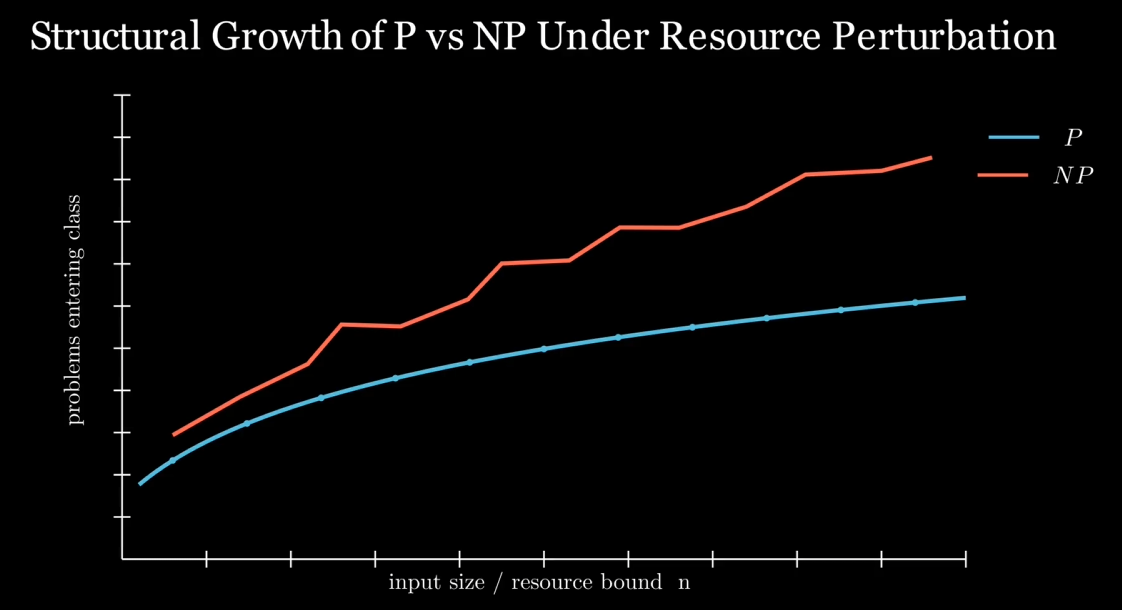
\includegraphics[width=0.7\textwidth]{Graph.png}
    \caption{A heuristic illustration of the growth of $P$ and $NP$ as a function of polynomial time bounds. The derivative $\Delta_C(p)$ corresponds to the slope of the curve at each point.}
    \label{fig:graph}
\end{figure}

\subsection{Critical Evaluation and Limitations}

Upon further reflection, several limitations became apparent.

Firstly, the derivative operator is not invariant under polynomial-time reductions. 
Techniques such as padding can artificially alter time bounds without changing the underlying computational difficulty of a language. 
This undermines the possibility that $\Delta_C(p)$ captures a canonical structural property.

Secondly, complexity classes are not typically analysed via cardinality or accumulation arguments. 
The framework implicitly treats the "number" of problems entering a class as meaningful, yet standard complexity theory is concerned with reductions and relative difficulty rather than counting arguments.

Thirdly, the framework does not circumvent known barrier results. 
Since $\Delta_C(p)$ is defined purely in terms of time bounds, any argument derived from it would relativise. 
By the Baker-Gill-Solovay theorem, relativising arguments cannot resolve $P$ vs $NP$.

Furthermore, broad structural arguments risk falling within the scope of the Natural Proofs barrier, which demonstrates that large, constructive properties cannot yield circuit lower bounds under standard cryptographic assumptions.

Therefore, while the framework is mathematically well-defined, it does not provide a rigorous separation mechanism.

For a derivative-based approach to succeed, it would need to satisfy at least two stringent conditions:

\begin{itemize}
    \item Invariance under polynomial-time reductions.
    \item Independence from oracle relativisation.
\end{itemize}

Additionally, it would require a structural property distinguishing $P$ and $NP$ that avoids largeness in the sense defined by Razborov and Rudich.

Identifying such a property would amount to discovering fundamentally new proof techniques beyond the known barriers.

\subsection{Structural Weakness of the Derivative Framework}

The central flaw in the derivative approach lies in its dependence on time-bound parametrisation rather than reduction-invariant structure.

Complexity theory is fundamentally comparative: languages are analysed via reductions rather than absolute time thresholds. Because the derivative operator $\Delta_C(p)$ is defined in terms of explicit polynomial bounds, it is sensitive to padding and encoding transformations.

If a language $L$ is padded to artificially inflate input size, its membership within $C_{\leq p(n)}$ may shift without reflecting any genuine change in computational difficulty. This demonstrates that the operator does not capture an invariant structural property of the class itself.

In effect, the framework measures artefacts of representation rather than intrinsic complexity.

A further limitation arises from the implicit reliance on counting arguments. The derivative interpretation suggests measuring how many problems "enter" a class as resources increase.

However, complexity classes are infinite sets of languages, and their cardinality does not significantly distinguish structural power. Both $P$ and $NP$ contain infinitely many languages, and cardinal growth does not correspond to computational hardness.

Thus, while the graphical heuristic suggests asymmetry, this asymmetry is not formally meaningful within the standard framework of complexity theory.

\subsection{Interaction with Known Barriers}

The derivative approach would necessarily relativise, since it is defined purely in terms of time-bounded membership. Any argument constructed from $\Delta_C(p)$ would remain valid relative to an oracle.

By the Baker–Gill–Solovay theorem, relativising techniques cannot resolve $P$ vs $NP$.

Furthermore, if the derivative operator were reformulated as a broadly applicable structural property, it risks satisfying the largeness and constructivity conditions characterising natural proofs. Under standard cryptographic assumptions, such properties cannot establish super-polynomial circuit lower bounds.

Thus, the framework fails not merely because it lacks rigour, but because it operates within the scope of already-identified barriers.

\subsection{Impact on the Direction of the Project}

This investigation proved valuable despite its limitations.

It clarified the importance of invariance under reduction as a necessary condition for any meaningful separation argument.

It also reinforced the significance of known barriers, particularly relativisation and natural proofs, by demonstrating how intuitive structural ideas can fail to translate into formal proof techniques.

Rather than weakening the project, this attempt strengthened its central thesis: that the difficulty of $P$ vs $NP$ lies not in a lack of intuitive asymmetry, but in the constraints imposed by proof methodology.

The derivative-based framework therefore represents an exploratory stage in the research process that deepened my understanding of both the problem and its barriers.

\subsection{Intellectual Outcome of the Attempt}

Although the derivative framework does not yield a separation, its failure was instructive.

It clarified that intuitive asymmetries between verification and construction are insufficient unless formalised through reduction-invariant structure. It also demonstrated how easily plausible structural arguments fall within the scope of known barriers.

Rather than weakening the project, this exercise strengthened its central thesis: the difficulty of $P$ vs $NP$ lies not in the absence of asymmetry, but in the rigidity of admissible proof methods.

\section{Development of Technical Skills}

\subsection{Learning \LaTeX}

\subsubsection*{Motivation}

At the beginning of the project, I chose to learn \LaTeX\ specifically for the EPQ.

Although unfamiliar with the system initially, I recognised that \LaTeX\ is the standard typesetting tool used in university-level mathematics and theoretical computer science.

Learning it during this project served both immediate and long-term purposes: improving the presentation quality of the dissertation and preparing for future academic study.

\subsubsection*{Initial Difficulties}

The learning curve was initially steep.

Simple formatting tasks such as inserting figures, managing references, and aligning mathematical expressions required learning new syntax and debugging compilation errors.

Understanding environments such as \texttt{figure}, \texttt{table}, and mathematical display modes required experimentation.

Errors were often cryptic, requiring careful reading of logs and incremental testing.

\subsubsection*{Technical Progression}

As the project developed, I became comfortable using:

\begin{itemize}
\item Mathematical environments for displayed equations.
\item Structured referencing via \texttt{natbib}.
\item Long tables using \texttt{longtable} and \texttt{tabularx}.
\item Controlled page layout and spacing.
\item Cross-referencing figures and sections.
\end{itemize}

This progression significantly improved the clarity and professionalism of the dissertation.

\subsubsection*{Impact on Mathematical Communication}

Learning \LaTeX\ influenced not only presentation but also mathematical thinking.

The requirement to structure arguments formally, define environments precisely, and organise sections coherently encouraged clearer logical progression.

In this way, the tool reinforced the discipline of mathematical writing itself.

\subsubsection*{Reflection}

Mastering \LaTeX\ during the EPQ transformed the project from a written report into a professionally formatted mathematical document.

It represents a transferable academic skill that will be used in future university study.

The decision to learn \LaTeX\ independently demonstrates both initiative and long-term academic preparation.

\subsection{Learning Manim for Visualisation}

\subsubsection*{Motivation}

The derivative-based framework required a visual illustration of how complexity classes might "grow" under incremental resource bounds.

Rather than sketching a diagram manually, I chose to generate a clean mathematical graphic programmatically.

This led to learning Manim, a mathematical animation engine commonly used for visualising abstract mathematical concepts.

\subsubsection*{Learning Process}

I had no prior experience with Manim.

Over approximately three hours, I read the official documentation in order to understand:

\begin{itemize}
\item Creating coordinate axes.
\item Plotting functions.
\item Labelling graphs.
\item Exporting static frames from animations.
\end{itemize}

The goal was not to master animation broadly, but to produce a precise visual representation suitable for inclusion in the dissertation.

\subsubsection*{Technical Outcome}

Using Manim, I generated a visual comparison between two abstract growth curves intended to represent heuristic behaviour of $P$ and $NP$ under changing polynomial bounds.

The resulting graphic was exported and incorporated into the dissertation as Figure~\ref{fig:graph}.

\subsubsection*{Reflection}

Learning Manim reinforced the significance of exact visual communication in mathematics.

Rather than relying on informal sketches, generating the graph programmatically ensured clarity, symmetry, and reproducibility.

The process also demonstrated the ability to rapidly acquire and apply a new technical tool for a specific mathematical purpose.

\subsubsection*{Reflection}

Learning Manim reinforced the significance of exact visual communication in mathematics.

Rather than relying on informal sketches, generating the graph programmatically ensured clarity, symmetry, and reproducibility.

The process also demonstrated the ability to rapidly acquire and apply a new technical tool for a specific mathematical purpose.

\subsection*{From Curiosity to Technical Depth}

At the beginning of the project, my understanding of $P$ vs $NP$ was almost entirely conceptual.

As research progressed, I encountered increasing levels of technical abstraction --- oracle constructions, circuit complexity, arithmetisation, and proof barriers.

Apprehending these topics required moving beyond intuitive explanations and engaging with formal definitions and structural arguments.

The transition from informal understanding to technical depth was one of the most significant intellectual developments during the project.

\subsection*{Developing Mathematical Communication}

A major challenge was not only understanding complex material, but expressing it with precision.

Early drafts often contained excessive explanation or everyday language. Over time, I learned that mathematical writing requires:

\begin{itemize}
\item Economy of language.
\item Structural clarity.
\item Exact terminology.
\item Avoidance of unnecessary narrative.
\end{itemize}

Rewriting sections for conciseness was often more difficult than drafting them initially.

The goal shifted from "explaining everything" to explaining exactly what was necessary.

\subsection*{Managing Word Count Under Technical Constraints}

A recurring difficulty was managing the word count while preserving technical integrity.

Complexity theory arguments require definitions, context, and careful phrasing. However, the dissertation had to remain within prescribed limits.

This constraint forced prioritisation:

\begin{itemize}
\item Removing redundant explanation.
\item Compressing historical context.
\item Focusing on structural barriers rather than peripheral discussion.
\end{itemize}

Paradoxically, the restriction improved clarity by forcing disciplined argument structure.

\subsection*{Growth in Mathematical Maturity}

One of the most significant outcomes of the project was not a specific theorem or conclusion, but an increase in mathematical maturity.

Later in the project, I found that I could approach dense technical material more efficiently.

Arguments that initially seemed opaque --- particularly in the algebrisation chapter --- became structurally interpretable.

I began to recognise patterns in proof structure, rather than viewing each paper as isolated difficulty.

\subsection*{Understanding Failure in Mathematics}

Studying proof barriers altered my perception of mathematical failure.

At first, it seemed discouraging that major approaches were proven insufficient.

However, through engaging with relativisation, natural proofs, and algebrisation, I came to understand that eliminating classes of techniques constitutes progress.

The project therefore reshaped my understanding of what it means for mathematics to advance.

\section{Reflection on the Exhibition Evening}
The exhibition evening revealed a distinction between mathematical understanding and mathematical communication.

Several attendees described $P$ vs $NP$ as “the impossible maths question,” and asked why it mattered. While I was able to explain the formal definition clearly, I realised that translating structural complexity barriers into intuitive significance was more difficult.

This highlighted a limitation in my communication: I could articulate technical structure, but struggled to convey why the barriers themselves represent progress rather than failure.

The experience confirmed my technical understanding, but exposed a need to improve how I translate abstract reasoning into accessible explanation.

\subsection*{Public Perception of the Problem}

During the exhibition evening, several attendees approached the project with a recurring question:

\textit{"Why is this important?"}

Others referred to $P$ vs $NP$ as "the impossible maths question."

These reactions revealed a gap between the internal mathematical significance of the problem and public perception.

\subsection*{Explaining Importance to a General Audience}

Responding to these questions required reframing the problem in accessible terms.

Rather than describing oracle constructions or circuit lower bounds, I explained:

\begin{itemize}
\item The distinction between verifying a solution and finding one.
\item The implications for cryptography.
\item The relevance to optimisation and algorithm design.
\end{itemize}

This experience highlighted that understanding a problem technically is different from communicating its significance effectively.

\subsection*{On the Idea of "Impossible"}

The characterisation of $P$ vs $NP$ as "impossible" was particularly striking.

Through studying barrier results, I had learned that the problem is not known to be impossible --- rather, specific classes of proof techniques are insufficient.

The distinction between "unsolved" and "impossible" became clearer during these conversations.

Explaining that proof barriers refine approaches rather than prohibit solutions reinforced my own understanding of mathematical progress.

\subsection*{Impact on Personal Understanding}

The exhibition evening demonstrated that true mastery involves the ability to adapt explanations to different audiences.

While the dissertation required formal precision, the exhibition required conceptual clarity.

The process of translating complexity theory into accessible language strengthened my confidence in the material and deepened my ownership of the subject.

\subsection*{Recognition of Communication Limitations}

The exhibition evening revealed an important distinction between understanding and communication.
While I was confident in the mathematical content, explaining why the problem matters to a non-specialist audience proved challenging.
Questions such as “Why is this important?” exposed a gap between technical comprehension and accessible articulation.
This experience reinforced that mathematical maturity includes the ability to translate abstraction into meaningful context.

Although the exhibition evening confirmed my technical understanding of the material, it also exposed limitations in my ability to translate advanced concepts effectively.

When asked why the problem was important, I found it easy to explain verification versus search and implications for cryptography.
However, when attempting to describe proof barriers or structural limitations, I realised how difficult it is to communicate abstraction without oversimplifying.

This experience revealed that understanding a subject deeply does not automatically confer the ability to explain it clearly to non-specialists.

Recognising this gap was constructive rather than discouraging. It highlighted an area for further development: the skill of simplifying without distorting.

\subsection*{Final Reflection on the Exhibition}

The exhibition evening demonstrated that mathematical maturity has two components: technical precision and communicative adaptability.

While the project strengthened the former, the exhibition highlighted the need to persist in developing the latter.

In this sense, the public presentation wasn't merely a showcase of completed work, but an extension of the learning process itself.

The exhibition evening revealed a gap between technical comprehension and communicative clarity.
While I was confident explaining formal definitions, I initially struggled to articulate why the problem matters outside theoretical computer science.
Repeatedly being asked, “Why is this important?” forced refinement of explanation.
It required translation from structural barrier theory into broader implications for cryptography, optimisation, and computational feasibility.
This experience exposed a weakness in communicative framing rather than conceptual understanding.
Addressing this gap improved the dissertation's introduction and strengthened my ability to situate abstract mathematics within a wider intellectual context.

\section{Intellectual Development}

At the beginning of the project, I approached $P$ vs $NP$ as if it were a single difficult theorem awaiting a clever insight.

Through engagement with barrier results, I came to understand that the problem is constrained not merely by difficulty, but by the limitations of entire classes of proof techniques.

This shift --- from viewing the problem as unsolved to understanding why it resists solution --- represents the most significant intellectual development of the project.

I began to recognise that mathematical progress often consists not of solving problems, but of identifying structural limitations on how they may be solved.

\subsection{Development of Mathematical Communication}

One of the most continuous challenges was learning to write with precision rather than verbosity.

Early drafts contained explanations that were conceptually correct but inefficiently phrased. Polishing these sections required studying how professional mathematicians compress complicated ideas into minimal language without sacrificing rigour.

The word-count constraint, initially frustrating, forced deliberate prioritisation of structural argument over descriptive exposition. This process improved not only the clarity of the dissertation, but my understanding of what constitutes mathematically meaningful content.

\subsection{Encountering Conceptual Difficulty}

The Natural Proofs chapter exposed weaknesses in my background knowledge, particularly in circuit complexity. 

Understanding non-uniform models, circuit families, and pseudorandom functions required pausing the primary literature and building prerequisite foundations independently.

Although initially discouraging, this process marked a transition in how I approach unfamiliar material: rather than abandoning difficult sections, I learned to identify missing conceptual tools and acquire them deliberately.

\subsection{Reflection on the Independent Attempt}

The derivative-based framework was the most personally ambitious component of the project.

Although it does not yield a separation of $P$ and $NP$, the attempt clarified the importance of invariance, reduction-based reasoning, and barrier awareness.

The exercise demonstrated that generating ideas is easier than generating viable proof strategies. More importantly, it revealed that genuine mathematical maturity includes recognising when an approach is structurally insufficient.

This distinction --- between creative speculation and structurally admissible reasoning --- represents a key intellectual development.

\subsection{Impact on Future Study}

This project has fundamentally shaped how I approach mathematics.

Rather than seeking immediate solutions, I have developed a stronger appreciation for organizational constraints and methodological rigour.

The experience of learning LaTeX independently and engaging directly with primary literature has also prepared me for university-level mathematical study.

More significantly, the project confirmed that my interest lies not only in solving problems, but in understanding the frameworks that determine how problems may be solved.

\section{Concluding Evaluation}

\subsection{Evaluation of Research Approach}

In retrospect, my initial decision to engage directly with primary research papers before consolidating foundational material was inefficient.
Although this accelerated exposure to the depth of the field, it resulted in repeated pauses to learn prerequisite concepts such as circuit complexity, oracle constructions, and arithmetisation.
A more methodologically efficient approach would have been to systematically master textbook foundations (e.g., Sipser, Arora-Barak) before attempting barrier papers.
However, the premature exposure to advanced material had one unexpected benefit: it clarified the scale of the intellectual challenge early in the project and reframed my expectations away from solution-seeking toward structural understanding.
This shift was critical.
It transformed the project from an attempted resolution into an analysis of methodological limitation.

\subsection*{Personal Evaluation of the Project}

This project began with curiosity.

I knew almost nothing about the formal framework of $P$ vs $NP$, beyond its definition and historical reputation. The simplicity of its statement contrasted with the scale of its difficulty, and that contrast became the central motivation for my investigation.

Over the course of the project, my understanding deepened significantly. What initially appeared to be a single open problem revealed itself as a network of structural results, proof techniques, and limitations. Studying relativisation, natural proofs, and algebrisation transformed my perception of the question from "Why has nobody solved this?" to "What must a solution avoid?"

\subsection*{Growth Beyond Technical Knowledge}

Although I did not resolve any open problem, the project achieved something more meaningful on a personal level.

I learned how to read research papers strategically rather than exhaustively.  
I learned how to write with mathematical precision and economy.  
I learned that failure in mathematics does not signify stagnation, but rather serves as a process of refinement.

The most valuable development was not mastery of complexity theory itself, but an increase in mathematical maturity.

\subsection*{On Independent Exploration}

The derivative-based framework I developed did not produce a formal separation argument.

However, attempting to construct such a framework forced engagement with invariance under reduction, structural robustness, and known barrier constraints.

Its failure was instructive. It demonstrated concretely why intuitive structural analogies must satisfy strict complexity-theoretic conditions to be meaningful.

\subsection*{Final Reflection}
The EPQ was not undertaken to achieve a grade, but to understand a question that genuinely fascinated me.

Studying $P$ vs $NP$ did not provide answers, but it reshaped how I think about mathematical difficulty.

The problem remains open. The barriers remain intact. Yet the project achieved its aim: understanding not only what the problem asks, but why it is so resistant to solution.

In that sense, the investigation was successful.

If repeating the project, I would begin with secondary expository sources before approaching primary research papers. While immersion accelerated long-term understanding, a more structured progression would likely have reduced early inefficiencies.

\subsection{Final Evaluation Against the Research Question}

The refined research question asked:

\textit{What are the main theoretical barriers to resolving P vs NP?}
The project demonstrates that failure has not been due to lack of effort or computational ingenuity, but rather due to structural limitations embedded within proof methodology itself.
Relativisation shows that oracle-preserving arguments cannot suffice.
Natural Proofs demonstrates that large, constructive combinatorial properties are incompatible with standard cryptographic assumptions.
Algebrisation further extends these limitations to algebraic extensions of computation.
Together, these barriers suggest that the difficulty of $P$ vs $NP$ is not accidental but methodological.
The project therefore succeeds in clarifying why the problem remains unresolved, even though it does not resolve it.
This distinction between explanatory success and proof success marks the central intellectual outcome of the investigation.

\end{document}